\chapter{Introduction}
\chplabel{intro}

Vision is the process of making sense of the world
based on light that bounces off objects and into our eyes.
From these ever-changing two-dimensional patterns of light,
the visual brain has to infer the structure of a three-dimensional world
composed of distinct objects interacting in a myriad of ways.

Unlike some mental processes---%
for example, mentally computing a percentage tip and adding it to a bill,
or trying to reason out the best move in a game of chess---%
visual inference is a mental ability that we are not often consciously aware of.
Not only does it come naturally to the vast majority of people,
it is a process that we do not have much conscious access to.
Our conscious mind perceives the world in terms of objects
and their locations and patterns of motion,
leaving us unaware of all the computation and inference
required to get us there.

Due to this lack of conscious awareness of visual inference problems,
people---including experienced researchers---often underestimate their difficulty.
In 1966, Marvin Minsky and Seymour Papert famously assigned Gerald Sussman
and other students the summer project of developing an object recognition system \parencite{Papert1966}.
Yet it has taken researchers almost 50 years
to develop a system that can recognize anywhere near as many types of objects
in real-world situations as an average person can.
Over the past five years, the field of machine learning has succeeded on tasks
that ten years ago seemed insurmountable,
identifying a wide variety of objects such as animals, household objects, and faces
in realistic situations and contexts.\footnote{
  This task of attaching a category label to an object in the world
  is referred to as \emph{object recognition}, \emph{object classification},
  or \emph{object categorization}.
  Object classification refers specifically to determining a category label
  for an object.
  Object categorization is a less common term for the same problem.
  Object recognition is more general;
  while it has traditionally been used to refer to the same problem
  as the other two terms,
  it can also include other problems such as generating a sentence to describe
  a multi-object image (see \scn{learning-paradigms}).}
The key to their success has been to harness ideas from the field of neuroscience
about how neurons connect, learn, and work together
to process our visual environment.
The brains of humans, mammals, and other animals were the only systems
that we knew could solve these difficult problems,
so it stands to reason that they should be the main source of information
about how to solve them with machines.

This thesis continues that dialogue between neuroscience and machine learning,
but with a slightly different goal in mind.
I want to understand how the brain solves these problems,
by creating functional brain models
that can solve difficult object recognition tasks
in a biologically plausible manner.\footnote{
  I will often use the term ``biologically plausible'' in this thesis.
  It refers to a mechanism that the brain could reasonably implement,
  given what we know about physical and biological constraints.
  Biological plausibility is a continuum,
  with some mechanisms being more plausible than others.
  There are also limits to how precisely we can estimate biological plausibility,
  particularly if we are only describing the system down to
  a particular level of resolution.
  For example, we might describe a neuron model that qualitatively captures
  the high-level characteristics of neuron input-output relations
  as biologically plausible;
  that does not mean the model fully describes everything going on in the biology.
  Thus biologically plausible does not mean biologically detailed,
  though models that are more detailed should offer a more plausible description,
  since they are more constrained by the biology
  (assuming the details are accurate,
  and that the model is still able to accurately reproduce
  the high-level behaviour that the simpler model captured).
  }
To do so, I start with machine learning models,
since these are currently the best artificial systems
at reproducing the high-level object recognition abilities exhibited by people.
I then try to make them better brain models by adding biological detail,
while maintaining the accurate object recognition abilities
of the original machine learning model.
Through this process,
I hope to develop a better understanding of how the brain might work,
and what kinds of processes might be going on to facilitate
the high-level behaviours that seem so intuitive to us.
I also hope to continue to inspire machine learning research
by bringing in more ideas from neuroscience.
One of the main engineering applications of the work in this thesis
is to what is known as \emph{neuromorphic} engineering.
This field constructs computer hardware that more closely resembles
the mechanisms and structures seen in the brain.
The models in this thesis are potential software for this hardware.
By making computer implementations more similar to the brain,
we can better understand and simulate how low-level brain function
gives rise to high-level behaviour.
We also bring the high-level behaviour of computers more in line with brains,
both in terms of increased performance in real-world situations,
and in terms of the energy required to achieve this performance.


%% \section{Background}

%% % Very quick overview of the visual cortices

%% % Deep learning background
%% % Supervised learning, success in machine learning

%% % Many current models don't use spiking neurons
%% % - describe what a spiking neuron is, how it's different than rate

%% % Challenges of learning with spiking neurons


%% \section{Approach and novel contributions}

%% % Need for biologically plausible training



\section{Outline}

The first two chapters of this thesis provide general background from
the fields of computational neuroscience (\chp{compneuro})
and machine learning (\chp{ml}),
as they pertain to this thesis.
Readers familiar with either field
should feel free to skip the corresponding chapter entirely,
and refer back to it only as needed.
More specific background will be provided at the start of each content chapter.

There are three content chapters in this thesis,
each investigating a different method
of constructing spiking networks for object classification,
and each with different success criteria.
Each content chapter begins by providing a background literature review
specific to the chapter,
before presenting the methods used, the results, and discussion.
Each content chapter is thus meant to act like a stand-alone paper,
and can be read independently,
though occasionally they will reference details
from the background chapters or other content chapters.

The first content chapter (\chp{nef}) examines
single-layer feedforward networks with fixed encoding;
that is, the connection weights from the inputs to the hidden neurons are fixed,
and only the connections from the hidden neurons to the outputs are optimized.
This technique allows for rapid training of simple object-classification networks.
The chapter explores a number of methods both for choosing encoding weights
and decoding weights in these networks,
and shows that they translate well to spiking neurons.
The main drawback of these methods is that they are not powerful enough
to address larger, more difficult object-classification problems.

The second content chapter (\chp{spike}) addresses this shortcoming
by looking into deep (multiple hidden layer) spiking networks.
These networks require much more training,
but are able to perform well on large and difficult object-classification problems.
They have been well-studied by the machine learning community,
and this chapter examines how they can be trained for and run in spiking neurons,
as opposed to traditional rate-based neurons.
It proposes novel methods both for making spiking neurons differentiable for training,
and for adding noise during training to make the final network
more robust to the variability caused by spiking neurons.
It then demonstrates that these methods can scale to large and difficult problems.
One drawback to these methods is that they are a poor hypothesis for how
the brain might \emph{learn} to solve the object classification problem,
since they use a learning mechanism---the backpropagation algorithm---%
not believed to be feasible in neurons.
This shortcoming motivates the third and final content chapter.

The third content chapter (\chp{learning})
investigates how the brain might learn
deep spiking networks for object classification.
%% (\ie/ during early childhood development).
It focuses on the question of how neurons may implement supervised learning.
Neither of the methods examined in the previous chapters
provides a suitable answer:
the method of \chp{nef} only addresses shallow learning,
it does not allow learning on the earlier connection weights;
the method of \chp{spike} uses backpropagation for deep learning,
a method that relies on running synapses backwards in addition to forwards,
for which there is no known biological mechanism.
This chapter explores a recently established method---%
Feedback Alignment---%
that uses random feedback weights for deep learning.
It examines in detail what this method both is and is not capable of,
and addresses challenges to produce a fully spiking model in LIF neurons.

Finally, this thesis concludes
with a summary of the key contributions
and an outline of some possible areas of future work (\chp{conclusion}).

Links to the source code used to generate all the work in this thesis
are available in \app{source}.


%%%%%%%%%%%%%%%%%%%%%%%%%%%%%%%%%%%%%%%%%%%%%%%%%%%%%%%%%%%%%%%%%%%%%%%%%%%%%%%%
\chapter{Computational Neuroscience}
\chplabel{compneuro}

The field of computational neuroscience takes a
computational approach to understanding the brain,
by seeking to understand both what computations the brain performs,
and how elements in the brain (\ie/ neurons and synapses)
work together to facilitate these computations.

Computational neuroscience has traditionally, as a field,
taken a bottom-up approach,
beginning by studying individual neurons,
and then looking at how neurons can be combined into successively
larger and larger networks until meaningful behaviour emerges.
Contrast this with psychology and cognitive science,
which have taken a more top-down approach,
beginning by studying the behaviours of creatures,
and then trying to understand how the brain facilitates these behaviours
in terms of the higher-level functions of large brain areas.
This difference means that historically,
the bulk of the work in computational neuroscience has focused
on developing detailed mathematical models of individual neurons,
then small- to medium-sized networks.
It is only recently that these fields have begun to meet,
resulting in neurally-detailed models
that can reproduce organism-level behaviours.

This chapter provides both a brief summary of
the relevant biological details,
as well as the concepts and models from computational neuroscience
that are used or expanded on in this thesis.


\section{Biology}

In this thesis, I am specifically interested
in how the human visual system functions.
This section provides some relevant biological details,
both at the neural level and at the network level.
It is important to note that the models developed in this thesis
are still relatively basic when compared with
all the individual facts that have been documented about the visual system
(particularly those of monkeys and cats,
from which most of our neural data about these areas comes).
Thus, this section provides only the most basic biological facts
as are relevant to this thesis;
for a more comprehensive overview of the biology of the brain,
both at the single-neuron and network level,
see \textcite{Kandel2012}.


\subsection{Neuron physiology}

\begin{figure}
  \centering
  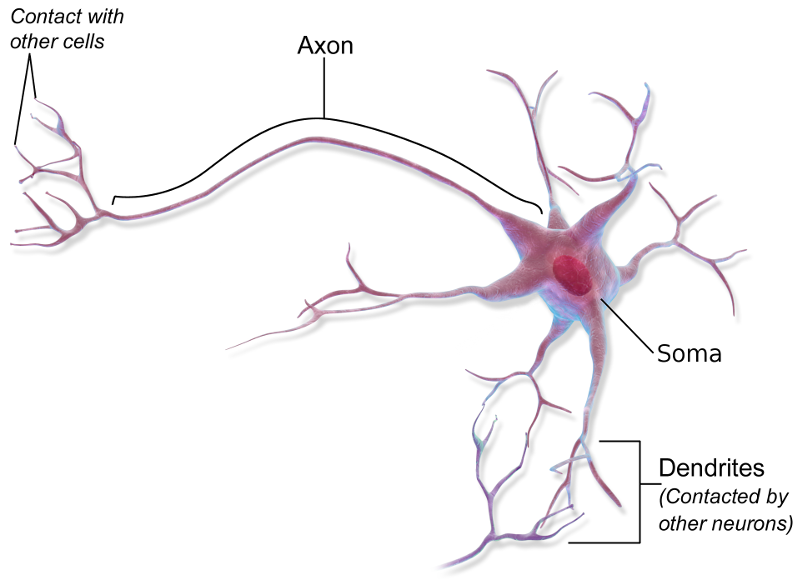
\includegraphics[width=4in]{neuron_small.png}
  \captionb{Cartoon of a neuron.}{
    A neuron receives input from other neurons via synapses on its dendrites.
    The dendrites transmit current to the soma,
    where electrical charge is integrated.
    If the neuron membrane becomes sufficiently polarized,
    it transmits an action potential (\aka/ spike) down its axon.
    This causes neurotransmitter to be released at the synapses,
    which then initiate currents in the dendrites of postsynaptic neurons.
    Image \textcopyright\textcite{BlausenNeuron} with modification, licensed under CC BY 3.0.
    }
  \figlabel{neuron}
\end{figure}

Neurons are only one of the many types of cells in the brain,
but they are the most discussed,
because they are the main computational entities.
Their basic function is simple:
neurons receive input from other neurons,
and if that input excites them sufficiently,
they will fire an action potential (\aka/ spike)
which propagates to other neurons.

A basic cartoon of a neuron is shown in \fig{neuron}.
Neurons can be divided into three parts: the dendrites, the soma, and the axon.
Neurons receive input currents via their dendrites,
which the dendrites then transmit or channel into the cell body,
called the soma.
When a neuron spikes, it sends current down its axon,
causing neurotransmitter(s) to release at the synapses,
which are connections from a neuron's axon
to the dendrites of other neurons.
This neurotransmitter release results in dendritic input currents
in these other connected neurons.

\begin{figure}
  \centering
  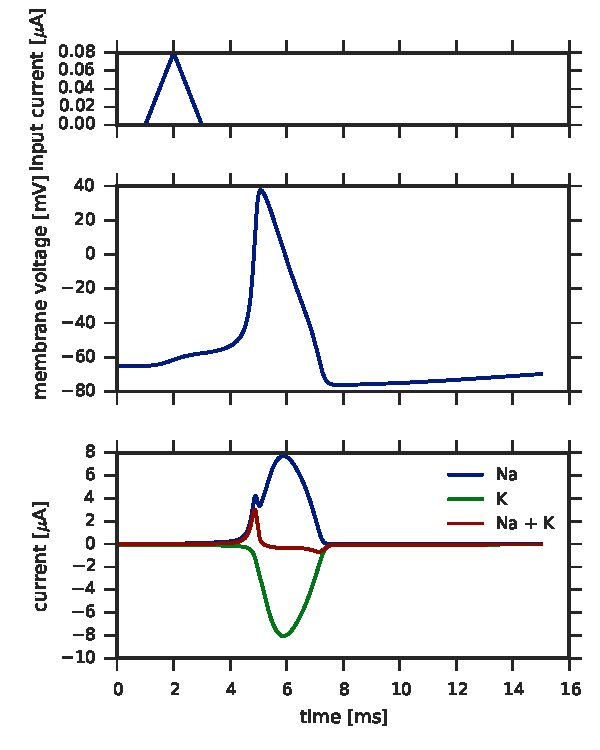
\includegraphics[width=4in]{hh_spike.pdf}
  \captionb{Spiking dynamics of a neuron.}{
    An external input current is applied at the soma of a neuron.
    It causes a slight ($\sim$10 mV) increase in the membrane voltage,
    which triggers a sufficient number of voltage-gated sodium channels
    to initiate a spike.
    The incoming sodium current increases the membrane voltage,
    which opens more sodium channels,
    causing an exponential increase in the membrane voltage
    (the leading edge of the spike).
    As the voltage nears its peak,
    it also triggers voltage-gated potassium channels,
    letting potassium ions out of the neuron and repolarizing it.
    The neuron then enters a hyperpolarized state (below its resting voltage)
    where the potassium channels slowly close
    and the sodium channels are inactivated.
    Only after a period of time (the absolute refractory period)
    can the neuron fire another spike.
    }
  \figlabel{neuron-spike}
\end{figure}

% The soma forms the main body of the neuron.
The soma is the main body of the neuron.
Computationally, it is where all the incoming currents from dendrites
are integrated,
and where the process of creating an action potential begins (\fig{neuron-spike}).
When a neuron is at rest, the soma has a negative charge;
this is called the resting voltage,
and is maintained by ion pumps that maintain a particular concentration of ions
(mostly sodium Na$^+$, potassium K$^+$, and calcium Ca$^{+2}$) inside the cell.
As currents arrive from the dendrites,
they begin to depolarize the cell.
When the voltage in the soma becomes high enough,
it begins to trigger voltage-activated sodium channels,
which allow sodium ions to enter the cell, further depolarizing it.
This process continues until the electrical gradient
due to the increase in sodium ions
opposes the chemical gradient due to the imbalance of sodium
inside and outside the cell.
This gives the neuron a much more positive charge
than when it is at its resting voltage.

This large depolarization also triggers voltage-gated potassium channels,
which begin to let potassium ions \emph{out} of the cell,
helping to repolarize it.
At the same time, the sodium channels inactivate.
The open potassium channels eventually bring the cell to below its resting voltage,
called the hyperpolarized state.
The sodium channels remain inactivated and the potassium channels remain open
for a while after the spike.
The combination of these factors makes it almost impossible
for the neuron to fire during this time;
this is called the absolute refractory period.
The change in ionic concentrations inside the cell is quite small
during a single spike,
but over the course of many spikes,
the ion pumps are needed to maintain the proper concentrations
of sodium and potassium.
Other currents, most significantly calcium currents,
are present in some neurons.

% axons
The rapid depolarization associated with an action potential
not only causes the somatic voltage potential to increase,
but also causes some depolarization in the parts of the axon
nearer to the soma.
This triggers sodium channels in that part of the axon,
resulting in more depolarization and
triggering sodium channels farther down the axon.
In this manner, the somatic spike triggers a voltage wave
that travels down the axon,
eventually triggering the synaptic vesicles near the ends of the axon
and causing them to release neurotransmitter(s).

Axons are responsible for transmitting long-range signals in the brain,
and thus vary widely in length,
depending on whether a particular neuron connects to nearby neurons
or to neurons in another brain area.
To facilitate long-range transmission,
axons are coated in myelin,
a substance composed mainly of lipids and thus a good electrical insulator.
This helps current to propagate down the axon.
The high proportion of fat makes myelin white;
bundles of axons are responsible for the ``white matter'' parts of the brain.
The ``grey matter'' on the other hand
is composed mainly of neuron dendrites, somas, and short-range axons.

% dendrites: active vs passive? role in computation?
Dendrites are thin processes that extend away from the soma
to connect to the axons of other neurons.
Their role is to transmit current from synapses with other neurons to the soma.
They were originally believed to only conduct current passively,
but research has shown that they have active conductance mechanisms
similar to those involved in spike generation and propagation down an axon
\parencite{Mel1994,Johnston1996}.
Dendrites are also traditionally believed to act linearly,
summing together inputs from many synapses across time and space,
and many computational models still treat them as such.
More recent studies \parencite[\eg/][]{Polsky2004} show that signal summation
in dendrites is more complex,
combining linear and nonlinear (sigmoidal) elements.

% synapses
Neurons are connected to one another by synapses,
connecting the axon of the presynaptic neuron
to a dendrite of the postsynaptic neuron.
When the presynaptic neuron spikes,
an electrical pulse travels down its axon to the presynaptic terminals
of all synapses on the axon.
These terminals contain synaptic vesicles filled with neurotransmitter;
the electrical pulse causes the vesicles to release neurotransmitter
into the synaptic cleft,
which is the small area between the presynaptic terminal
and the postsynaptic terminal.
This neurotransmitter activates receptors on the postsynaptic terminal,
which open, allowing current to flow into the postsynaptic cell.
The type of neurotransmitter used by the synapse depends on the presynaptic neuron.
All synapses on a neuron's axon release the same neurotransmitter
or combination of neurotransmitters; this is known as Dale's principle.\footnote{
  When Dale's principle was developed,
  it was believed that each neuron only produced
  one type of neurotransmitter.
  It was only around 1976 that evidence of cotransmission was discovered
  \parencite{Burnstock2004}.
  Nevertheless, Dale's principle remains a good guideline.
  For example, neurons are either exclusively excitatory or inhibitory
  based on the neurotransmitter(s) they release;
  no neurons play both an excitatory and inhibitory role
  to different postsynaptic cells.}


\subsection{Visual system anatomy}

% ventral and dorsal streams

The human visual system performs many functions;
it is not limited to object recognition.
Other functions include estimating object shape, depth, motion (tracking),
and physical characteristics (\eg/ smoothness, hardness) for tasks like grasping,
as well as identifying landmarks and estimating ego-motion for navigation.
The way that many researchers think of the visual system
has been shaped by what is known as the ``two-streams'' hypothesis \parencite{Goodale1992}.
The hypothesis is that the visual system can be roughly divided
into two streams, known as the dorsal and ventral streams.
The ventral stream is sometimes called the ``what'' pathway,
and is associated with object and landmark recognition.
The dorsal stream is sometimes called the ``where'' or ``how'' pathway,
and provides information to inform motor actions related to objects,
such as grasping an object or avoiding an obstacle.


\begin{figure}
  \centering
  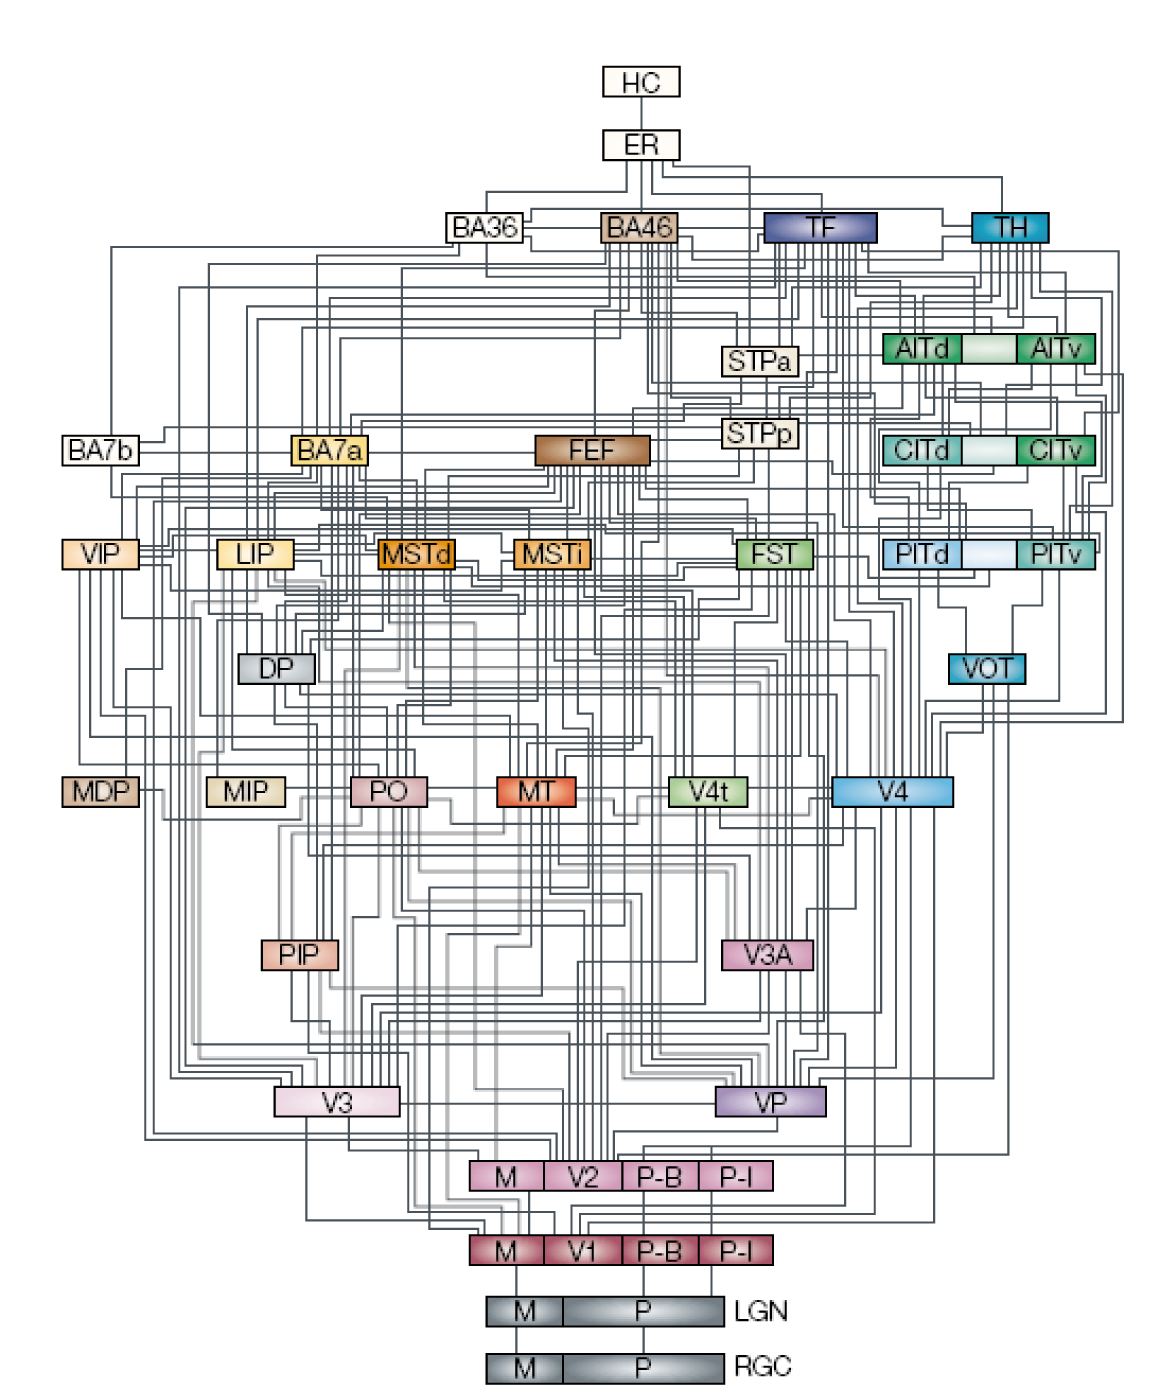
\includegraphics[width=5in]{felleman_vanessen.png}
  \captionb{Hierarchy of the visual cortex of a macaque.}{
    Reproduced from \textcite{Felleman1991},
    depicting connectivity between brain areas in macaque visual cortex.
    Most of the connections have been demonstrated to be reciprocal.
    The ventral stream is on the right,
    culminating in the inferior temporal (IT) areas (AIT, CIT, PIT).
    The dorsal stream is on the left,
    culminating in the intraparietal (IP) areas (VIP, LIP).
    This figure does not show the strength of connections.
  }
  \figlabel{visual-hierarchy}
\end{figure}

% VanEssen visual hierarchy diagram
\fig{visual-hierarchy} is reproduced from \textcite{Felleman1991},
a famous paper examining connectivity in the visual cortices of macaques,
which are known to have similar visual system organization to humans.
The input to the system is at the bottom: the retinal ganglion cells (RGC).
They are already a few steps in from the photoreceptors that transduce
light into neural signals,
and represent a compressed version of the raw photoreceptor input \parencite{Nassi2009}.
The RGCs relay their information through the lateral geniculate nucleus (LGN),
a part of the thalamus.
While some authors do not discuss computational properties of the LGN,
treating it simply as a relay station \parencite[\eg/][]{Nassi2009},
others have found that some LGN cells introduce temporal lags into the signal \parencite{Vigeland2013},
which would be useful for representing motion information \parencite{Adelson1985}.

The next step in visual processing is primary visual cortex (V1).
V1 neurons begin to separate stimuli in a number of ways,
being tuned for changes in contrast (edges), depth, motion, colour, and other properties.
V2 is the next visual layer, it plays a significant role in image segmentation,
specifically representing object contours and border ownership \parencite{Kruger2013}.
It is at this point that the visual system begins to separate
into dorsal and ventral streams.
The ventral pathway continues to V4 and then on to inferior temporal (IT) cortex,
by which point neurons are responsive to object categories.
The dorsal pathway continues to MT and MST---%
both very involved in motion processing---%
before continuing on to intraparietal (IP) cortex
which localizes objects in \ddd/ space and informs motor planning
for actions like grasping.
\textcite{Kruger2013} provides a review of the key visual areas
and their role in computation.

\fig{visual-hierarchy} illustrates how interconnected the visual areas are.
While the dorsal and ventral streams are visible on the left and right, respectively---%
with a high level of connectivity within the streams---%
there is also significant connectivity between the streams.
The functional role of the connections between the streams
remains largely unclear.
Computational models of object recognition---%
including those examined throughout this thesis---%
rarely account for these connections.


\section{Neuron models}

Many of the seminal results in computational neuroscience
are mathematically detailed models of how neurons operate.
Perhaps the most famous of these is the Hodgkin-Huxley model
of the squid giant axon \parencite{Hodgkin1952}.
More recently, the numbers of available neuron models has blossomed,
and current models used in literature range from simple
binary threshold units \parencite{Stocks2001a} (the simplest possible rate-neuron model),
to complex multi-compartmental models
that account for detailed dendritic morphologies \parencite[\eg/][]{Markram2015,}.

For large models of neural systems that hope to reproduce high-level behaviour,
single-compartment neuron models are still the norm.
These models treat the neuron as a single electrical compartment,
combining the dendrites, soma, and axon.
Multi-compartmental models, on the other hand,
model different parts of the neuron as different electrical compartments,
and include equations how the activities of different compartments affect each other.
Models can range from having two compartments
(typically one for the dendrites and one for the soma),
to having thousands of compartments.
The more compartments a model has,
the more computing power it takes to simulate it,
and the more complex its behaviour becomes.
For these reasons, models that seek to reproduce behaviour
predominantly use either single-compartment neurons,
or simpler models that do not model the electrical activity of the neuron at all.
These models are what I will discuss here,
and use throughout the thesis.

Single-compartmental neuron models can be divided along two dichotomies:
1) the rate-based versus spike-based dichotomy;
and 2) the static versus dynamic dichotomy. %\footnote{
  %% There are many other ways to divide and categorize neuron models,
  %% for example single-compartment versus multi-compartmental models.
The rate versus spiking distinction has to do with whether
the output of the neuron model is a continuous value (a firing rate)
or a discrete value (a spike).
Most neurons in mammalian cortex communicate via spikes,
so spiking neuron models are typically considered more physiologically realistic.\footnote{
  There are limited places in the mammalian brain---%
  for example horizontal cells in retina---%
  where neurons communicate via gap junctions,
  and thus could transmit something more akin to a continuous value
  than a discrete spike.}

The static versus dynamic distinction denotes whether the model has
internal dynamics,
such that the output at the current point in time is conditional in some
respect on the time history of the neuron,
or static, such that the output is completely independent of the past
and only dependent on the instantaneous neuron input.
Dynamic neuron models have some form of state,
that is internal variables that evolve over time,
and are not directly computable from the present input to the model.
They are typically expressed using differential equations.
For static models, the output is a function of the current input only,
and thus they do not require differential equations to express them.

% describe rate response function (I-F curve)
It is important to note that the static/dynamic dichotomy does not necessarily
refer to whether the neuron is being used as a static nonlinearity
(evaluated at a single point in time on an input \emph{value})
or as a dynamic nonlinearity (evaluated over a period of time on an input \emph{signal}).
Static neurons can be evaluated dynamically,
simply by evaluating them (independently) on the input value at each successive point in time.
For dynamic neurons, however, there is no general way to evaluate them statically,
since their input at any point in time depends on their internal state,
which is a dynamic process that evolves over time.
For some dynamic neuron models,
we can determine a firing rate response curve
(\aka/ I-F response curve, rate response function),
which maps every constant value for the input current
to a constant firing rate output.
This can be determined analytically (\eg/ \eqn{lifrate}),
or empirically by applying a constant input current
and measuring the rate of the output spikes
(this can even be done in real neurons in vitro).
Many neuron models will not output spikes at a constant rate,
even for a constant input,
due to changing internal dynamics.
For these neuron models,
the rate-response function only captures part of the model,
and will be different depending on the state of the model
and how it is measured or calculated.


\begin{table}
  \centering
  \begin{tabular}{l|l|l}
            & \multicolumn{1}{|c}{\textbf{Rate}}
            & \multicolumn{1}{|c}{\textbf{Spiking}} \\\hline
    \textbf{Static}
      & Sigmoid                   & Poisson spiking              \\
      & Rate LIF                  &                              \\\hline
    \textbf{Dynamic}
      & Adapting rate LIF         & LIF                          \\
      & Sigmoid with state        & Hodgkin-Huxley               \\
  \end{tabular}
  \captionb{Rate vs. Spiking and Static vs. Dynamic neuron model dichotomies.}{
    Neuron models can either transmit information via continuous firing rates (rate-based),
    or via discrete spikes (spike-based).
    They can either have no internal state (static),
    or have their response affected by internal dynamical systems (dynamic).
    }
  \tablabel{neuron-dichotomies}
  %% \vspace{6pt}
\end{table}

\tab{neuron-dichotomies} shows how a few example neuron models fall across
these dichotomies.
In the static rate category, we have models that take in
a continuous value and output a continuous function of that continuous value.
This includes most of the nonlinearities used in machine learning
(such as sigmoids or rectified linear units),
as well as the analytic firing rate for the LIF neuron model (see \scn{lif}).
In the static spiking category, we have models that output a discrete (binary)
function of their continuous input.
This is mainly Poisson-spiking neurons,
which fire probabilistically based on their instantaneous firing rate,
such that the probability of firing at the current time is
independent of past firings.\footnote{
  Poisson spiking can also be applied to a dynamic rate model,
  such that the probability of spiking is independent, but the spike rate is a
  dynamic process \parencite[\eg/][]{Lillicrap2016}.}
Dynamic rate models have an internal state that also affects their continuous output,
in addition to the input.
This includes the analytic LIF rate model with adaptation,
which has an internal adaptation parameter that grows when the neuron is active
and discounts the firing rate.
It also includes sigmoid neuron models that have an underlying voltage
that is dynamically related to the neuron inputs;
such models have recently been applied by \textcite{Guergiuev2017}
when learning deep networks subject to biological constraints.
Finally, the dynamic spiking category includes the LIF neuron model,
as well as the Hodgkin-Huxley model,
as well as more complex multi-compartmental models.

Within the category of spiking models,
we can further distinguish between
models that output instantaneous spikes (\eg/ LIF),
and models that output spikes which vary across time (\eg/ Hodgkin-Huxley).
Another possible distinction would be between models
that output stereotyped spikes,
where the size of each spike is exactly the same,
and those that output variable-sized spikes.
Models of cortical neurons that output instantaneous spikes (\eg/ LIF)
almost always output stereotyped spikes.
This is because spikes in cortical neurons are nearly identical
in terms of magnitude, duration, and shape,
and it is widely believed that none of these factors carry information.
Even among models that have spikes that vary across time (\eg/ Hodgkin-Huxley),
the spike magnitude, duration, and shape are quite consistent between spikes.
Therefore, most spiking cortical neuron models have stereotyped spikes.
Modelling the spike separately from the rest of the neural dynamics
allows for a separation of time scales;
the result is that extra computational resources are not required
to model the spike trajectory,
the details of which are stereotyped and thus of little interest \parencite{Abbott1999}.


\subsection{The integrate-and-fire neuron model}

The integrate-and-fire (IF) neuron \parencite{Lapicque1907}
was one of the first computational models of a neuron.
This model was developed before researchers were able to measure
the electrical and chemical changes happening in a behaving neuron,
and is based simply on the idea that the neuron membrane
can be modelled as a capacitor that stores charge over time \parencite{Abbott1999}.
As the name implies, the IF model has two main behaviours:
1) it integrates current over time (by means of the capacitor);
and 2) when the voltage has reached a threshold, it fires.
Additionally, the model may or may not include a leak term:
a resistor in parallel with the capacitor that allows charge
to ``leak'' out over time.
The model with leak term is typically referred to
as the leaky integrate-and-fire (LIF) model.
While ``integrate-and-fire (IF) model'' can refer to either the leaky or non-leaky model,
in this thesis I will use it to refer specifically
to the non-leaky version of the model.


\subsubsection{The non-leaky integrate-and-fire (IF) model}
\scnlabel{if}

We wish to identify how the neuron's membrane voltage evolves over time,
and from this identify when the neuron spikes.
The charge $Q$ across a capacitor is given by $Q = VC$,
where $V$ is the voltage across the capacitor and $C$ is the capacitance.
Differentiating this with respect to time,
we find that the membrane voltage $V(t)$ of the neuron is governed by
\begin{align}
  C \diff{V(t)}{t} = J(t)
  \eqnlabel{ifdiff}
\end{align}
where $J(t)$ is the input current to the neuron over time,
and $C$ is the membrane capacitance.
(Remember that current is the time derivative of charge.)

\eqn{ifdiff} shows that the IF neuron simply integrates
the input current over time.
We still need to identify when the neuron spikes.
To do this, we define a threshold voltage $\Vth$.
When the voltage passes this threshold, the neuron fires.
This comes from a key fact in neurophysiology:
once the neuron voltage passes a threshold,
the neuron begins firing a spike,
and once this firing process begins,
it is almost impossible to reverse.

Finally, we define a reset procedure:
once the neuron has fired a spike,
the membrane voltage is reset to the resting potential $\Vrest$.
This again comes from physiology:
after a neuron spikes,
other ionic currents (typically potassium)
kick in and bring the membrane voltage back towards the resting potential.

Some integrate-and-fire models may also model an absolute refractory period:
a time $\tref$ for which the voltage is held at the resting potential $\Vrest$
after a spike.
In cortical neurons, post-spike potassium currents are strong enough
that it is practically impossible for the neuron
to fire another spike for a period of time.
This time is called the absolute refractory period.
We model this by holding the membrane voltage at $\Vrest$
for a length of time $\tref$.


\subsection{The leaky integrate-and-fire (LIF) model}
\scnlabel{lif}
% Citation: Knight1972
% Citation: Gerstner and Kistler 2002? Koch1999?

The leaky integrate-and-fire (LIF) model \parencite{Lapicque1907,Knight1972,Koch1999}
takes one additional physiological factor into account:
Neuron membranes are not perfect capacitors,
rather they slowly leak current over time,
pulling the membrane voltage back to its resting potential.
Thus, we model the membrane as a capacitor and resistor in parallel.
This gives the neuron some ``forgetting'':
in the absence of any input, the membrane voltage will return to its
resting potential.

The LIF dynamics are captured by the following equation:
\begin{align}
  C \diff{V}{t} = -\frac{1}{R}(V - \Vrest) + J(t)
  \eqnlabel{lifdifffull}
\end{align}
where $R$ is the membrane resistance,
and the other parameters are the same as in the IF model.
The resetting procedure is also identical to the IF model.


\subsubsection{Normalized model}

The LIF model has a number of parameters:
$C$, $R$, $\Vrest$, $\Vth$.
We can normalize the model to reduce the number of parameters,
while keeping the full dynamics of the original model.
Specifically, we manipulate the model
so that the normalized voltage lies in the range $[0, 1]$,
with a normalized resting potential of zero
and normalized firing threshold of one.

First, we multiply \eqn{lifdifffull} through by $R$:
\begin{align}
  \taurc \diff{V}{t} &= -V + \Vrest + R J(t)
\end{align}
where $\taurc = RC$.
Then, letting $\bar V = (V - \Vrest) / (\Vth - \Vrest)$
and $\bar \Vrest = \Vrest / \Vth$:
\begin{align}
  \taurc (\Vth - \Vrest) \diff{\bar V}{t} &= -(\Vth - \Vrest) \bar V + R J(t) \nonumber\\
  \taurc \diff{\bar V}{t} &= -\bar V + \frac{R}{\Vth - \Vrest} J(t) \nonumber\\
  \taurc \diff{\bar V}{t} &= -\bar V + \bar J(t)
  \eqnlabel{lifdiff}
\end{align}
where the firing threshold for the new equation is $\bar \Vth = 1$,
the voltage is reset to $\bar \Vrest = 0$,
and $\bar J(t) = \frac{R}{\Vth - \Vrest} J(t)$.
Observe that $\bar J(t)$ is simply a linear transformation of $J(t)$.
Thus, \eqn{lifdiff} retains all the dynamics of \eqn{lifdifffull} for a scaled input,
but with only one parameter $\taurc$.

Note that $\bar V$ and $\bar J$ are both unitless quantities.
In this thesis, we work exclusively in this unitless space,
and often refer to $\bar V$ and $\bar J$ simply as $V$ and $J$,
despite the fact that these quantities are not actually voltages or currents.
This simplifies the mathematics,
without limiting the generality of our models.


\subsubsection{Rate equation}

\eqn{lifdiff} describes exactly when the model neuron will spike
for a given input current $J(t)$.
However, sometimes we only care about the spike rate,
that is, how many times per second the neuron will spike
for the given input current.

For the LIF model, we can determine the analytical firing rate
for a constant input current.
We do this by determining the inter-spike interval (ISI),
that is the time between one spike and the next.
Then, the firing rate is given by the inverse of the ISI.

Given a constant input current $J(t) = j$,
we can solve \eqn{lifdiff} to find the neuron voltage over time:
\begin{align}
  V(t) = (V(0) - j) e^{-t / \taurc} + j
  \eqnlabel{lifvoltage}
\end{align}
assuming no spikes are fired.
We want to know how long it takes for the voltage to rise from $V(0) = 0$
to $V(t) = 1$.
This will only occur if $j > 1$.
Substituting into \eqn{lifvoltage} and solving for $t$:
\begin{align}
  t &= -\taurc \log\left(-\frac{1}{j}\right) \text{ .}
\end{align}
Adding in the refractory period and inverting,
the spike rate $r$ for the LIF neuron is given by
\begin{align}
  r = \frac{1}{\tref - \taurc \log\left(1 - \frac{1}{j}\right)}
  \eqnlabel{lifrate}
\end{align}
if $j > 1$, and zero otherwise (since the neuron is silent).


\section{Synapse models}
\scnlabel{synapses}

In addition to modelling internal neural dynamics,
it is also important to model the dynamics of the synapses
that connect neurons to one another.
The most significant functional effect of synapses is
as a low-pass filter on the spikes passing through them.
A spike in the presynaptic neuron elicits an extended current pulse
in the postsynaptic neuron.
This pulse can be viewed as a low-pass-filtered version
of the presynaptic spike.

The simplest model of a synapse is as a first-order lowpass filter.
The impulse response of a filter describes how the filter responds to
an infinitesimally short input of unit integral, called an impulse.
This idealized impulse is also reasonable model of a spike,
thus the impulse response also describes what the postsynaptic current
will look like in response to a presynaptic spike.
The impulse response of the first-order lowpass filter is:
\begin{align}
  h(t) = \frac{1}{\taus} e^{t / \taus}
  \eqnlabel{expo-synapse}
\end{align}
where $\taus$ is called the synaptic time constant,
and relates to the length of time the postsynaptic current is spread over.
Since the impulse response is an exponential function,
it is known as the exponential synapse model.

\textcite{Mainen1995} found that a second-order lowpass filter
is a better model of a synapse.
The impulse response of this filter is given by
\begin{align}
  h(t) = \frac{t}{\taus^2} e^{t / \taus} \text{ .}
  \eqnlabel{alpha-synapse}
\end{align}
This function is known as the alpha function,
and thus the model is called the alpha synapse model.
%% Again, $\taus$ is the only parameter of the model,

Both of these models are current-based synapse models,
meaning that they explicitly model the current that results from a spike
in the postsynaptic neuron.
Other current-based synapse models exist;
a popular one is the double-exponential model,
which is similar to the alpha synapse but with two time constants,
allowing more control over the rise and fall of the impulse response.\footnote{
  The double-exponential model with both time constants set to the same value
  reduces to the alpha synapse.}
Many of the other, more realistic synapse models are conductance-based,
meaning that they model the conductance of the neural membrane at the synapse.
The current into the neuron depends on both the conductance
and the voltage across the membrane;
the latter changes as the synapse becomes active.


\section{Rate codes, population codes, and timing codes}
\scnlabel{codes}

%  - Difference between rate and temporal codes is actually in the freq.
%    of fluctuations in the firing rate. Not related to independence.
%  - In a pure rate code, Poisson spiking would be equivalent to constant-ISI
%    spiking, whereas in \eg/ an NEF network, the fluctuations produced by
%    Poisson spiking could be interpreted as meaningful by downstream neurons.
%  - My idea: for a particular (constant) stimulus, a rate code would have
%    constant FR, whereas a timing code would have fluctuating FR?
%  - Example of distinction: rate code for stimulus intensity versus rank-order
%    timing code (\eg/ Bhattacharya2010). Rate code still has some temporal
%    aspects, for example neurons with higher input intensity will fire first.
%    This is what allows first-to-spike metrics to work even in networks trained
%    with rate neurons.
% difference between rate and timing codes is whether changing phase of
% regular spike train affects results?

One of the aims of computational neuroscience has been to determine
how the brain represents---or encodes---information.
To this end, researchers have proposed a number of different
\emph{coding schemes} that neurons could use to encode information.


\subsubsection{Rate versus timing codes}

One dichotomy differentiates between rate coding and temporal coding.
In a rate code, only the firing rate (\ie/ number of spikes)
of a neuron over a period of time matters.
An archetypal example of a rate code
is motor neurons in the peripheral nervous system.
A muscle's contraction is based on the number of spikes per unit time,
thus only the rate of motor neuron spikes is important \parencite{Gerstner1997}.
In a temporal code, the \emph{time} of individual spikes is also important.
An archetypal example of a timing code is in the early auditory system \parencite{Gerstner1997},
where precise spike timing helps to localize sounds \parencite{Chase2006}.

The exact definitions of rate and temporal codes are not clear,
and vary from author to author \parencite{Dayan2001}.
For example, a neuron may fire a number of spikes in quick succession,
and then be silent.
Compare this with a second neuron, that fires the same number of spikes,
but spread evenly over a given period.
One way to view this is that both neurons have the same firing rate,
but the one has all its spikes near the start of the period,
in which case the timing of the spikes is important.
An alternative view says that the \emph{instantaneous} firing rate of
the first neuron changes over the period,
whereas that of the second neuron remains constant,
and it is only this instantaneous firing rate that matters.
This points to one problem with only looking at the overall firing rate
(\ie/ number of spikes) of a neuron over a period:
it is not clear what period we should count over.
In real neurons,
the period of time that matters for counting spikes depends on parameters like
the membrane time constant $\taurc$ of the postsynaptic neuron.

For this reason, neuroscientists will often distinguish
between rate and timing codes
based on the frequency of the changes in the instantaneous firing rate.
If the rate fluctuates rapidly,
and these fluctuations contain information about the stimulus
(they are not simply spurious variation or ``noise''),
then the code is said to be temporal; otherwise it is a rate code.
Again, there is ambiguity as to how fast the firing rates must fluctuate
to be considered temporal.
One way to define this is relative to the stimulus.
Fast-changing stimuli can trigger fast changes in the firing rate of neurons,
whether they are using a rate code or a temporal code.
If we define a temporal code as having meaningful firing rate fluctuations
at a faster time scale than changes in the stimulus,
we can differentiate between codes that have fluctuations
because they are using them for coding,
and those that simply have fluctuations triggered by the stimulus.
By this definition,
neurons using a temporal code will have a fluctuating firing rate
in response to a constant stimulus,
whereas neurons using a rate code will have a non-fluctuating firing rate.


\subsubsection{Population coding}

Both rate codes and temporal codes describe
the encoding properties of individual neurons.
We can also ask about the coding properties
of a group (\aka/ population) of neurons.
The concept of \emph{population coding} describes when a representation
is distributed across many neurons in a population,
such that the represented value cannot be decoded from only the activities
of a few neurons.

To illustrate, the simplest way of extrapolating the idea of rate or temporal
coding to more than one neuron
would be to have many neurons all implementing the same code.
That is, all neurons will fire similarly when representing a given value
(they have similar \emph{tuning}).
This creates a large degree of redundancy between neurons.
Instead, population coding has each neuron represent a different aspect
of the represented value.
For example, if we want to represent head direction,
we have neurons that represent the head fully turned to the left,
others that represent fully turned to the right,
and still others for centred, and others for values in between.
The direction that a neuron is most active for is called its preferred direction.
Each neuron has some variance, that is, it will fire for head directions
close to its preferred direction, as well.
The farther the actual head direction is from a neuron's preferred direction,
the less it will fire.
By using the activities of all neurons in the population,
we can decode the head direction quite accurately.

At the population level,
we can distinguish between codes that take advantage of synchrony between neurons
and those that do not.
This can be facilitated for example by \emph{coincidence detection},
where a postsynaptic neuron will only fire if the spikes of two
of its input neurons are coincident,
that is, they fall within the same (small) temporal window.
Here, we see another distinction between temporal and rate coding schemes:
Only temporal codes can take advantage of correlations
between individual spikes of neurons.
Rate coding schemes, on the other hand,
can only take advantage of synchrony between neurons in terms of
synchronized fluctuations of their instantaneous firing rates,
since they do not have the temporal precision to co-ordinate individual spikes.

%% Therefore, the fundamental distinction between rate and temporal codes
%% is that in a rate code, the whole system will function as well or better
%% if all spiking neurons are replaced with ideal rate-based approximations.
%% With temporal codes, the timing of individual spikes matters,
%% so they will no longer function properly when using rate-based neuron models.


%% \subsubsection{Sparse and distributed representations}

%% When discussing coding at the population level,
%% another important distinction is between sparse and distributed representations.


\section{The Neural Engineering Framework (NEF)}
\scnlabel{nef}

The Neural Engineering Framework (NEF, \textcite{Eliasmith2003}
is a theory that connects neural-level computations
with higher-level algorithmic descriptions.
Specifically, it describes how neurons can perform vector computations,
which can then be built upon to create increasingly complex systems,
for example Spaun \parencite{Eliasmith2012}.
It has three main tenets:
1) representation, how neurons represent a real-world value;
2) transformation, how neurons compute (static) functions on represented values;
and 3) dynamics, how neurons can implement dynamical systems or functions.

The core of the Neural Engineering Framework is based on population coding.
Specifically, it extends a method proposed by \textcite{Salinas1994}
on how linear least-squares can be used to find linear decoders for a
population of neurons.
This idea can be summarized succinctly as
``nonlinear encoding, linear decoding''.
Here, we will focus on the first two tenets: representation and transformation.


\subsubsection{Representation}

The core idea behind the NEF is that a ``population'' of neurons
can be viewed as representing some value.
This could either be a value in the real world
(such as an animal's current head direction)
or a purely internal value
(such as the sum of three and seven when mentally computing $4 \times (3 + 7)$).
In the core NEF, each population represents a vector $\vect x$,
but this can be extended to representing things like
scalar- and vector-fields, too.

Each neural population has a set of \emph{encoders} $\mat E$,
which map from the space of values that the population can represent
(called the state space, of dimension $d$)
to the space of neural activities (called the neuron space, of dimension $n$).
The mapping is nonlinear:
\begin{align}
  a_j(\vect x) = G_j\left(\alpha_j \sum_i E_{ji} x_i + \beta_j\right)
\end{align}
where $\vect x$ is the vector value that the population is encoding,
$a_j$ is the activity of neuron $j$,
$G_j(\cdot)$ is a rate-based neural nonlinearity
transforming input currents into firing rates,
$\mat E$ is a $n \times d$ matrix of encoders,
and $\alpha_j$ and $\beta_j$ are scalar gain and bias terms, respectively.
Often, neurons in the NEF are modelled as LIF neurons,
in which case $G_j$ is given by \eqn{lifrate} for all neurons.

To decode information from the population,
we find linear decoders $\mat D$,
which when multiplied by the neural activities $\vect a(\vect x)$,
will yield our state-space value $\vect x$.
Typically, we choose decoders that minimize the squared error
$\|D \vect a(\vect x) - \vect x\|_2^2$.
Ideally, we would minimize this across all possible values of $\vect x$;
in practice, we sample the space of $\vect x$ at $m$ points,
called evaluation points.
Given our $m \times d$ matrix of evaluation points $\mat X$,
and the corresponding neural activities at each evaluation point $\mat A$,
we can find the least-squares optimal decoders as
\begin{align}
  \mat D = (\mat A^T \mat A)^{-1} \mat A^T \mat X \text{ .}
\end{align}
In practice, some neurons may have similar activity patterns,
making this an ill-conditioned problem.
Additionally, we typically want to put a penalty on large decoders
to reduce the effects of variability in the spiking neurons on the decoded value.
To address these problems, we typically regularize the problem
(see \scn{dec-regularization}).


\subsubsection{Transformation}

Since the number of neurons in the population $n$
is typically much larger than the number of dimensions $d$ in the encoded vector $\vect x$,
the neural population not only contains information about $\vect x$,
but also about possible functions of $\vect x$.
We can decode a function $f(\vect x)$ from the population
by finding decoders $D_f$ that minimize the squared error
$\|D_f \vect a(\vect x) - f(\vect x)\|_2^2$.
This results in a similar least-squares optimization problem as before,
but replacing the matrix of evaluation points $\mat X$
with a matrix of targets $\mat Y$.
This method can be used to decode arbitrary functions from the population.
The accuracy with which a given function can be decoded depends
on the characteristics of the function
(\eg/ higher frequency changes are more difficult to decode),
the tuning curves of the neurons,
and how these two factors relate.


\subsubsection{Discussion}

%%  - encoding/decoding model is rate-based. This is not to say NEF models
%%    use only rate coding; firing rates can change quite quickly, thus
%%    exhibiting something more akin to temporal coding. However, the
%%    fundamental model is of neurons as rate-based. Furthermore, all neurons
%%    are treated as independent. Synchrony between neurons is not exploited,
%%    in fact it is discouraged, since it would cause correlated noise between
%%    neurons, and here we treat all spiking ``noise'' as independent.
One observation about the encoding model is that it is rate-based.
To find the decoders, we use the rate response function of the neurons.
This does not mean that NEF models use traditional rate coding;
firing rates can vary quite quickly,
and one can design models---for example an oscillator---%
where neurons fire in quick bursts, for which the timing is important.
NEF networks cannot take advantage of synchrony between neurons;
any correlations between neural firing will only result in
increased variability (noise) in the decoded output.
Furthermore, NEF networks function equally well or better
when rate-based neurons are used instead of spiking neurons.
This suggests that these networks use what is fundamentally a rate code,
albeit one that can change quickly.

%%  - Neurons are heterogeneous, play large role in what functions we can decode
An important aspect of NEF networks is that neurons are heterogeneous
in terms of their encoders and biases,
and thus respond differently to input stimuli.
This heterogeneity is what allows neurons to not only encode
different aspects of their input signals
(something that can also be done with noisy homogeneous neurons, see \textcite{Hunsberger2014}),
but compute nonlinear transformations of these signals.
The exact nature of this heterogeneity has a significant effect
both on what signals can be represented,
and what transformations can be computed.
Representation and transformation do not always go hand in hand;
for example, a population whose neurons are all tuned to the sum of two inputs
is not able to represent the individual signals,
but is able to compute a transformation such as the square of their sum.
What types of heterogeneity are best for computing particular functions
has not been well examined.
\scn{nef-encoding} will look at what types of encoders are good
for performing object classification tasks.


\section{Neuromorphic hardware}

Neuromorphic engineering is broadly concerned with creating artificial systems
that work like biological neural systems,
particularly in terms of their physical implementation.
The term was coined by Carver Mead in the late 1980's,
and refers to both digital and analog hardware
that is organized in a more brain-like manner
than traditional computer hardware \parencite{Mead1990}.
One of the core ideas behind neuromorphic systems
is parallel distributed processing;
neuromorphic systems organize computations at a neural level,
and pay particular attention to facilitating fast communication between
neural processing units.
This differs from other parallel distributed systems
like graphics processing units (GPUs),
which are typically optimized for independent parallel computations
and have poor communication between units.

Neuromorphic systems can be either digital or analog.
Digital systems, such as SpiNNaker \parencite{Furber2013} and TrueNorth \parencite{Merolla2014},
use the same basic components as traditional computers
(even using the same chips in some cases),
but optimize connectivity and communication for neural systems.

Analog systems embrace the fundamental analog nature of electrical systems,
and construct systems using core components that are analog instead of digital.
On some systems (\eg/ NeuroGrid, \textcite{Benjamin2014}),
neurons are modelled using analog circuits.
This is extremely energy efficient compared with digital circuits,
since as little as one RC circuit can represent
and update a neuron membrane voltage with leak,
which would require multiple bits and multiple updates per time step
on digital hardware.


%%%%%%%%%%%%%%%%%%%%%%%%%%%%%%%%%%%%%%%%%%%%%%%%%%%%%%%%%%%%%%%%%%%%%%%%%%%%%%%%
\chapter{Machine Learning}
\chplabel{ml}

The field of machine learning (ML) is concerned with how computers
can learn to perform various tasks,
and is a sub-branch of the field of artificial intelligence (AI).
AI addresses the problem of how to get machines
to do ``intelligent'' things.
Initial approaches were focused on how to program this desired intelligence,
and grew out of fields like optimization and control theory.
One drawback to this initial approach is that the programmer would need
to be able to formulate specific instructions telling the machine how to
act in different circumstances.
This led to \emph{rule based systems},
which are successful at some tasks,
but for other tasks it is incredibly difficult to determine
an explicit set of rules to guide behaviour.
For example, how would you choose rules to differentiate between
the visual stimuli of a cat and a dog?
You can begin by trying to make rules to distinguish between different
characteristic features;
for example, differences in the appearances of ears, noses, mouths, and so on.
However, it is very hard to come up with rules that cover
even the majority of situations,
and promising rules may prove to be fragile to changes in viewing angle,
viewing distance, or environment.
The reason it is so difficult to come up with rules for this situation
is that recognizing objects is something that people do subconsciously.
We cannot think of explicit rules because we do not have them,
not in the same way that we have rules for doing mental math, for example.
Rather, our visual system has been bombarded over time with
millions of seconds of ever-changing stimuli,
and learned to process these stimuli in such a way that we can do everything
from distinguishing different types of objects,
to judging the depths of obstacles in our environment.

Machine learning was born when researchers started asking whether
we can get machines to learn these implicit ways of operating, too.
Rather than programming in a set of rules or commands,
can we have the machine learn its own program, so to speak.
This is often described as a \emph{data-driven} approach:
give the machine a general structure for the problem,
and a lot of data,
and let it \emph{learn} a way to solve the problem.
Empirically, there is no general structure that works well across
different types of problems,
and much of the research in machine learning goes into
what kinds of structures, and what kinds of learning procedures,
work best for a particular problem or group of problems.

One of the most prolific sub-fields in machine learning has been that of
artificial neural networks (ANNs).
ANNs take inspiration from the brain
by defining a ``neuron'' (or node) as the fundamental unit of computation.
Typically in an ANN,
a neuron will take a (linearly) weighted set of inputs,
and then pass this through a (static) function to obtain the neuron's output.
An ANN can have many such neurons,
and much of machine learning is concerned with how to adjust the parameters of the model
(typically the weights on each neuron's inputs)
such that the model as a whole obtains the desired output.
Additional difficulty comes from the fact that we do not want our system to
only perform well on the stimuli that we train it on,
but also on stimuli that it has not seen before.
It is relatively easy to memorize a set of desired input and output pairs,
and given one input produce the desired output.
It is much more difficult to generalize what has been learned to new
stimuli in an ``intelligent'' manner,
and this generalization problem is the core problem of machine learning.

This chapter will summarize the ANN sub-field of machine learning,
particularly those aspects concerned with solving object classification problems,
which have been one of the core problems used to demonstrate the abilities of ANNs.
I will briefly summarize the development of ANNs,
before focusing on some of the key pieces related to their modern practice.


\section{Machine learning basics}

Early efforts in artificial intelligence were driven by theory:
Researchers would take what they knew about the problem
and use it to develop algorithms and rules to address that specific problem.
It soon became clear that for many problems,
it was extremely hard to explicitly write out
all the rules that would be needed to solve that problem.
For example, traditional computer vision approaches have relied on
detecting specific hand-defined features in an image.
This can work reasonably well for problems like tracking moving objects,
where simple features can be combined with the principles of motion
to keep track of an object from one frame to the next.
For problems like object recognition, however,
it is almost impossible to explicitly define good features and rules.
To tell a cat from a dog from a boat from a truck,
one would need to design feature detectors for things like ears, eyes,
sails, wheels, and so on,
and then define rules about how these relate for different types of objects.
One would quickly have hundreds of features and rules,
and would have to hand-tune each one to work properly on the data.


\subsection{Goal}

Machine learning takes a data-driven approach.
Rather than explicitly define good features and rules,
the goal of machine learning is to \emph{learn} them from the data.
Specifically, we want to learn a function
that is able to perform the desired computation on new data points
(\ie/ different from the ones used for learning).
This is called \emph{generalization},
and is what allows a machine-learning system to be deployed in the world.
If the system only performed well on stimuli that it has already seen,
then unless we can show it every possible stimulus it will ever see
(which is impossible for high-dimensional stimuli, such as images),
the system will always perform poorly on new stimuli.
If, however, the system is able to generalize
from the training stimuli to similar stimuli,
then it can perform well on novel stimuli too.

The desired computation of a machine learning system
is defined implicitly both by the available training data,
and by the learning paradigm.
The latter is the focus of the next section.


\subsection{Learning paradigms}
\scnlabel{learning-paradigms}

The learning paradigm defines both what information
we have available to learn from,
and what the desired output of the system is.
There are three main paradigms:
supervised learning, unsupervised learning, and reinforcement learning.
The main way these paradigms differ is in terms of what type of error signal
is provided to the learner.

In supervised learning,
we have both the desired inputs and outputs to the system,
and we wish to learn an input-output mapping.
It can be separated into regression problems, which have continuous outputs,
and classification problems,
which have binary outputs (representing membership in different categories).
The error signal is defined based on how far the system's output
is from the desired output.

In unsupervised learning,
we have input data (\eg/ images), but no desired outputs.
Rather, we implicitly define an output based on the input data.
Types of unsupervised learning include
clustering, which attempts to group the input data into sets,
and dimensionality reduction, which attempts to represent the data using
fewer dimensions than the original representation.
The error signal is defined based only on the input.
For example, for dimensionality reduction,
we wish to create a system that can take an input and represent it with fewer dimensions,
but still re-create the input from this representation.
In this case, the error signal could be how far this re-creation
is from the original input.

Finally, reinforcement learning has a more temporal aspect:
given a current state of the environment,
the system must choose an action,
which determines (perhaps probabilistically) the next state of the environment.
Certain environmental states are rewarded,
while others are punished (negative reward) or neutral (no reward).
The system wants to achieve maximum total reward over time.

While these are the main categories of learning problems typically studied in ML,
this is not an exhaustive list.
Other paradigms exist, such as semi-supervised learning,
where some data points are labelled and others are not
(thus falling between supervised and unsupervised learning).
Supervised learning is still the dominant paradigm in object recognition.
As datasets grow larger and thus the cost
of having fully labelled datasets is higher,
object recognition will likely move to incorporate more
semi-supervised and unsupervised methods,
and even reinforcement learning
(\eg/ when object recognition is part of a larger problem,
such as winning at video games \parencite{Mnih2013}).
That said, this thesis focuses only on supervised learning.

Within supervised learning, there are two traditional kinds of problems:
regression problems and classification problems.
The difference is in the output of the system.
Regression systems output one or more continuous values
(computing a vector-valued function on the input),
whereas classification systems compute a single discrete-valued output
(representing the class-label of the input).
More recently, there has been increased interest
in problems that go beyond these two categories.
One example is predicting multiple labels for an image---%
for example corresponding to many objects in an image---%
or determining verb-like correspondences between objects \parencite{Karpathy2015}.
This can be expanded to generating captions for images,
where the model output is a sentence describing the image
\parencite{Karpathy2015,Xu2015}.
This thesis will focus on classification problems,
which is the typical paradigm used when performing object classification.


\subsection{Basic components}

Each machine learning system can be described in terms of four components:
\begin{enumerate}
  \item Dataset/Problem:
    The set of data that is available to learn from,
    which implicitly defines the problem. In the case of supervised learning,
    this is a set of input/output pairs; in unsupervised learning, it is only
    inputs; in reinforcement learning, it is an environment that defines the
    set of possible states and which states produce which rewards.
  \item Architecture:
    How our learner is constructed,
    namely what are the parameters being learned,
    and how is the system output determined
    given these parameters and an input value.
  \item Objective function:
    The metric by which we evaluate a particular set of parameters.
    In supervised learning, two such functions are often used,
    one for training and one for testing (evaluation).
    The training objective function is called a \emph{loss function},
    where zero loss indicates ``perfect'' performance,
    and any positive loss indicates how far we are from perfect performance.
  \item Optimization algorithm:
    The algorithm by which we minimize the loss function.
    Ideally, this algorithm will find the set of parameters that result
    in the smallest possible loss value (\ie/ the global minimum)
    on the given dataset (in a reasonable amount of time).
\end{enumerate}
These four components completely characterize the learning problem:
if one describes all these components in full detail,
then any other person should be able to perfectly reproduce the result.
Since the choice of these components completely determines
the capabilities of a learner,
all machine learning research looks at at least one of them.
Typically, to compare between different ML systems,
researchers will fix the dataset and evaluation objective function,
and vary the architecture, loss function, and optimization algorithm.
This allows a system to obtain a score on a particular dataset
relative to other systems.
Of course, each dataset may only provide a limited view of the capabilities
of a particular system (some more than others),
and it is common to test systems on multiple datasets.


\subsection{Overfitting and underfitting}

Given our goal of generalizing well to new data,
there are two main pitfalls in ML: underfitting the data and overfitting the data.
Underfitting the data occurs when our system is not able
to capture the (implicit) function we are trying to learn.
One way this can happen is if the architecture is not powerful enough
to represent the function.
A simple example of this would be if we have linear network,
but are trying to learn a nonlinear regression function:
no matter how good our learning methods are,
there is no set of model parameters with which our chosen architecture
will be able to compute the desired function.
Another way that this can happen is if our learning methods
are not able to find good parameters for our chosen architecture,
even though they do exist.
Recent work has shown that shallow networks
can often perform as well as deep networks,
but deep networks are still preferred in most cases
because it can be difficult or impossible to learn the shallow networks
directly from the data \parencite{Ba2014}.\footnote{
  The way that the shallow networks were learned
  was to first learn a deep network,
  then to train a shallow network to reproduce the outputs
  of the penultimate layer of the deep network
  (\ie/ the inputs to the softmax layer).}
This is an example of a situation where the architecture
(in this case the shallow network)
is theoretically powerful enough to represent the desired function,
but it cannot be trained well using traditional learning methods
(it can only be trained by trying to mimic the deep network).

Overfitting occurs when our model begins to learn
relationships in the training data
that are not useful for the problem at hand.
This happens because the architecture
is too powerful for the dataset in some way,
and rather than learning general features about the data
(that will apply to new stimuli),
it learns idiosyncratic features about specific stimuli
that apply only in the case of those examples.
An extreme example is a learner that simply memorizes every training example,
returning the correct answer for all training examples
(as provided during the supervised training),
but outputs a random output for all other stimuli.
This learner will perform perfectly on the training set,
but is simply guessing on all other stimuli,
and thus has not learned to generalize at all to new examples.
Characteristics of this extreme behaviour can be seen in otherwise successful learners,
where some parameters in the model may adjust to accommodate
idiosyncrasies in particular stimuli;
in this way, the model has memorized features about these stimuli
to be able to identify them,
but in a way that will not generalize to other similar stimuli.

Overfitting is relatively simple to detect:
it occurs when the model performs significantly worse
on novel stimuli than on training stimuli.
The presence of such a generalization error
indicates that the model has learned features about the training set
that do not apply outside the training set.

Detecting underfitting is not as straightforward.
The simplest measure is that if the network is not achieving zero training error,
then it is not able to fully model the desired function,
and is underfitting to some degree.
However, that assumes that the training data is perfect,
in that all of the labels are correct and unambiguous.
It also relies on current architectures being powerful enough
to fully capture all the nuances of the target function,
which is often not the case.
Another way to detect underfitting is by assuming that
any model that is not overfitting is underfitting.
This is a good assumption,
because there is a very limited window in which a model is
perfectly capturing a relationship;
it is almost always either underfitting or overfitting.
Furthermore, overfitting is not entirely bad;
improving the training performance on a model that is already overfitting
can still improve the performance on new examples.
Overfitting simply means that the model is beginning to pick up
spurious relationships in the training data.
Further training may still help it pick up some true relationships,
in addition to more spurious relationships.

To address underfitting,
we either want to make the architecture more powerful
(\eg/ increase the number of parameters),
or improve the learning methods so that we can find better parameter values.
Early machine learning was often unsuccessful on even relatively simple datasets
because computers were simply not powerful enough to allow for
the larger models needed.
Convolutional neural networks have been successful
because they make the parameters easier to learn.

To address overfitting,
we need to limit the architecture in some way,
such that it learns more good patterns within the data and fewer spurious ones,
or expand the dataset such that learning spurious correlations is less advantageous.
In simple cases, where the model is much too large for the dataset,
simply reducing the number of parameters can help,
particularly if done in a way that incorporates some prior knowledge of the problem.\footnote{
  For example, in visual recognition problems,
  having local connectivity in the first layer of a deep neural network
  can improve performance.
  This is because low-level visual features are local,
  and limiting connectivity pushes the network to pick up on
  true short-range correlations rather than spurious long-range ones.}
However, the number of parameters can only be reduced so much
before the model begins underfitting.
At that point, we need to begin limiting the values of parameters in some way:
this is called regularization.
Simpler forms of regularization simply put a cost
on having larger parameter values,
which prevents the learner from putting too much weight
on some correlations over others,
and thus relying too heavily on any one feature.
Dropout is a newer form of regularization for neural networks
that probabilistically silences neurons,
again preventing the learner from only relying on a few features (see \scn{dropout}).
Finally, expanding the dataset (see \scn{dataset-usage})
can help with overfitting,
since the learner has to perform well on more training examples,
thus putting more constraints on the parameters.


\subsection{Dataset usage}
\scnlabel{dataset-usage}

The dataset has two uses:
training the system (finding the optimal parameter values),
and testing the system (evaluating the parameter values).
Ultimately, we are interested in determining how well a learner \emph{generalizes},
that is, how well it performs when exposed to stimuli it has never seen before.
In supervised learning, datasets are typically divided into
distinct training and testing subsets.
This way, the learner can be tested exclusively on examples
it has never seen during training.

There are many parameters related to the architecture, loss function,
and optimization method that are not learned,
but rather must be chosen \emph{a priori};
these are known as \emph{hyperparameters}
(examples include learning rates, the size of the model,
and the initial values of the learned parameters).
Since the choice of these parameters
can have a great effect on the generalization error,
it is important to choose them without knowledge of the test set.
Otherwise, one may end up tuning the hyperparameters
to the specific test set being used,
such that it becomes a poor estimator of generalization error
since the learner will perform less well on examples outside the test set.
To account for this, it is common to hold another subset of the data
out of training,
called the \emph{validation set}.
This subset can be used to help tune hyperparameters;
for example, a simple scheme to find the optimal learning rate
might try many possible learning rates
and pick the one that results in the best performance on the validation set.
The resulting learner would then be applied to the test set,
and the performance on that set would be a good estimate
of generalization error.

%% We can also use the validation set to help us detect overfitting

Just as the brain has many synapses to allow it to solve difficult problems,
modern ML methods have many parameters to make them powerful enough to solve
real-world problems.
To tune this many parameters,
it is important that datasets are sufficiently large,
providing a wide range of stimuli such as one might encounter in the world.\footnote{
  As an example, try to imagine all the images that one might take
  with even a small, low-resolution camera (\eg/ $256 \times 256$ pixel),
  This would include every sort of variation on every common object,
  seen from any angle in any lighting condition.
  Then, since each object would only take up maybe a quarter of the frame,
  one could include all possible combinations of these objects.
  The total number of such images is astronomical.}
Given a core dataset, one can expand the number of training images
by creating variations on each image:
this is called \emph{dataset augmentation}.
For example, one might include small translations (shifts) of each image,
as well as left-right flips.
This can significantly help reduce the chances of overfitting
by increasing the diversity of the dataset,
helping it to better characterize the stimulus space.


\subsection{Objective functions}
\scnlabel{objective-functions}

In supervised learning,
the \emph{objective function} or \emph{loss function} of a network
defines the quantity that we wish to optimize,
relating the actual outputs of the network $\vect y$
to the desired outputs of the network $\vect y^*$.
It is often described as a \emph{cost} or \emph{loss}
that we wish to minimize.
This cost, in simple terms, describes how poorly our network performs
on the training data set.
Some common loss functions for classification are described in \scn{nef-decoding}.

One important distinction is between loss functions and error functions;
for regression problems, these functions are often one and the same,
but in classification problems, they are typically different.
An error function quantifies how much error a network makes;
for classification, this is typically the number of examples incorrectly classified
divided by the total number of examples.
An example is considered incorrectly classified
if the output with the highest value is not the correct output.
The classification loss, on the other hand,
depends on the values of the outputs.
For example, a loss function might penalize (\ie/ have non-zero loss)
for an example if the network output for the correct class is not as high as desired,
or if the margin between the correct output and next most active output
is not as large as desired.
This means that many examples that are correctly classified
will still have non-zero loss.
Overall, this pushes the classifier to not only get the answer correct,
but to get it correct by a significant margin,
which ideally makes the classifier more robust
and better able to generalize to new inputs.
The loss function is also continuous and differentiable,
whereas the error function can be discrete;
this makes the loss function more easily optimizable,
since the derivative(s) can be used in the optimization.


\subsection{Datasets}
\scnlabel{datasets}

Collecting and annotating datasets
for supervised learning of object classification
is not a trivial task.
To support development of new machine learning models and methods,
and to facilitate comparison between models and methods,
there are a number of standard datasets
publicly available and commonly used in the machine learning community.
Here, I summarize all the datasets that are used at some point
in this thesis (see \tab{datasets}),
which are five of the most common object classification datasets.

\begin{sidewaystable}
  \begin{tabular}{lrrrrl}
    Dataset & Image size & \# classes & \# train & \# test & Description\\\hline
    MNIST & $28 \times 28$ & 10 & 60k & 10k & Handwritten digits from zip codes\\
    SVHN & $32 \times 32$ & 10 & 72k & 24k & House numbers from Google Street View\\
    CIFAR-10 & $32 \times 32$ & 10 & 50k & 10k & Some types of animals and vehicles\\
    CIFAR-100 & $32 \times 32$ & 100 & 50k & 10k & Animals, objects, vehicles, trees, etc.\\
    ILSVRC-2012 & $256 \times 256$ & 1000 & $\sim$1281k & 100k & Animals, objects, buildings, landscapes, etc.\\
  \end{tabular}
  \captionb{Summary of datasets used in this thesis.}{}
  \tablabel{datasets}
\end{sidewaystable}

\begin{figure}
  \centering
  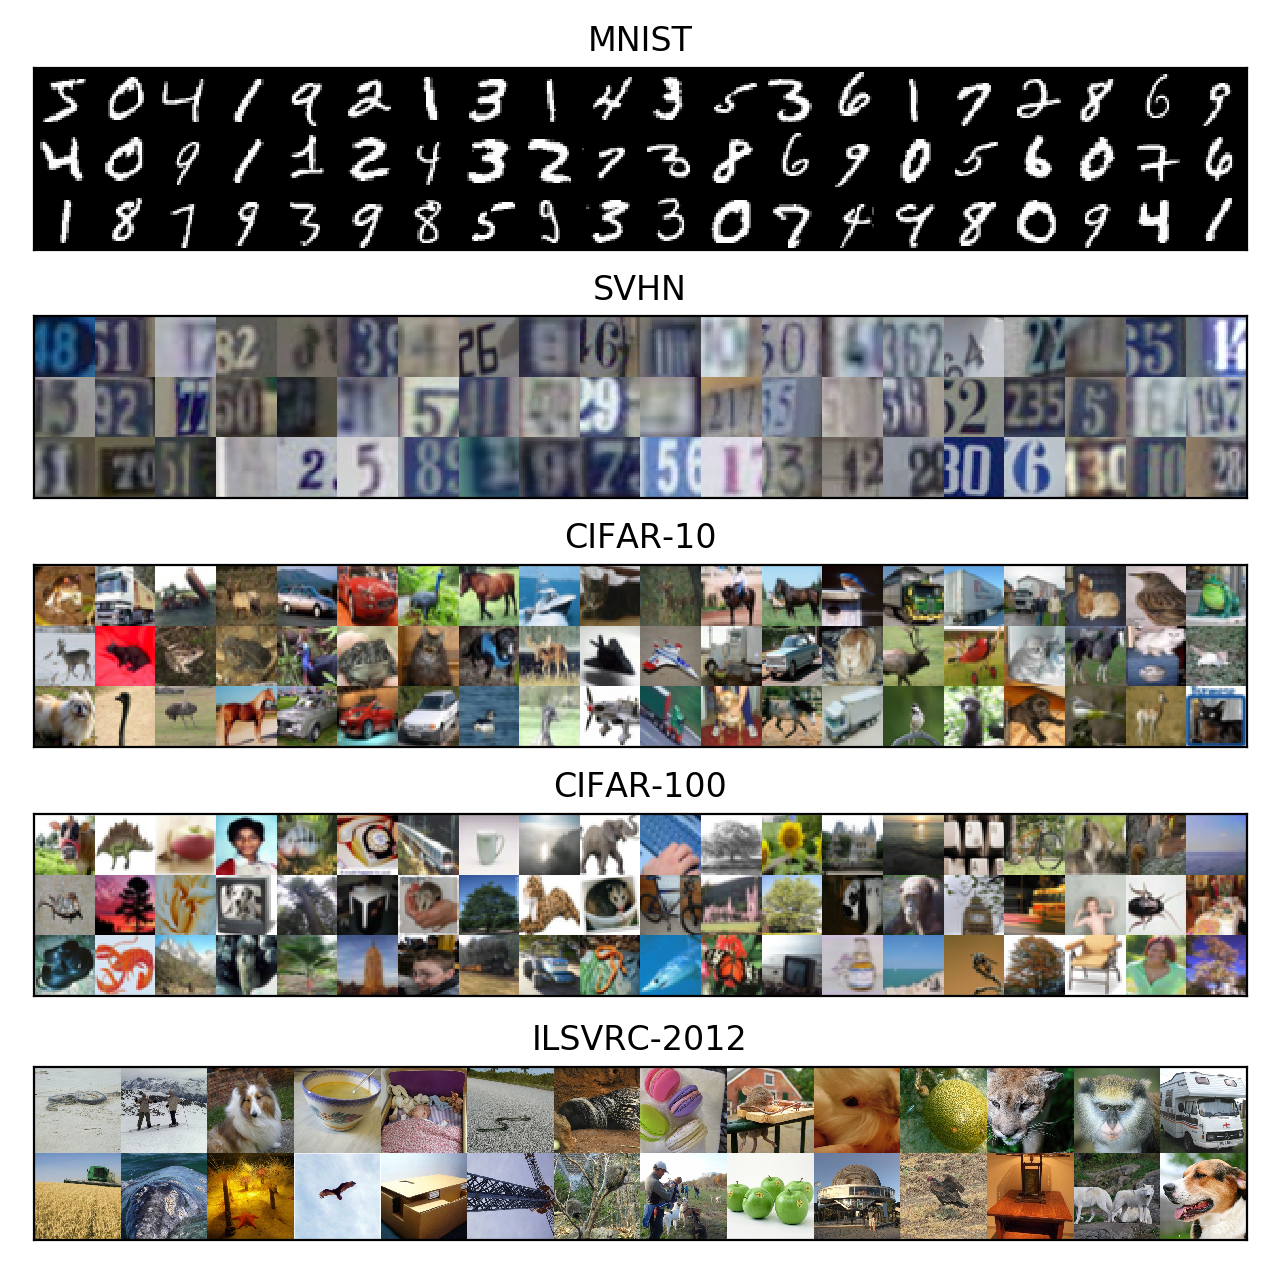
\includegraphics[width=6.35in]{datasets.png}
  \captionb{Example images from datasets used in this thesis.}{}
  \figlabel{datasets}
\end{figure}

The MNIST dataset \parencite{Lecun1998} is a collection of handwritten digits
(taken from US zip codes written on envelopes).
The digits have been heavily preprocessed such that each image
contains exactly one centred digit in high contrast greyscale
(essentially black and white).
Optical classification of handwritten characters is a challenging problem,
and the first true success on this problem by \textcite{Lecun1998}
marked a turning point in machine learning.
While the dataset is no longer challenging for state-of-the-art methods,
it is still commonly used as a first benchmark for novel models and methods.
Its relatively small size (by modern standards)
allows for expedient training even with slower methods
(\eg/ online learning and spike-based methods).

The SVHN dataset \parencite{Netzer2011} is also composed of digits,
taken from images of house numbers on Google Street View.
They show large variation in the styles of digits,
as well as in the backgrounds, lighting, colours, and contrast.
They have been preprocessed such that each image is centred
on a digit (the target digit for classification),
however images often contain whole or partial digits to the sides
(distractor digits).
This makes the dataset considerably harder than MNIST,
but still relatively easy compared to datasets composed of objects.
State-of-the-art algorithms achieve under 2\% error,
which is better than the estimated human error of 2\% \parencite{Netzer2011}.

The CIFAR-10 and CIFAR-100 datasets \parencite{Krizhevsky2009}
consist of small ($32 \times 32$ pixel) images from
10 or 100 different categories, respectively.
All the images are taken from the Tiny Images Dataset \parencite{Torralba2008},
and are in full colour.
Despite being the same size as the SVHN dataset,
these datasets are considerably harder:
Human performance on CIFAR-10 has been estimated at 94\% accuracy \parencite{Karpathy2011},
and state-of-the-art algorithms get around 96\% accuracy \parencite{Springenberg2015,Graham2015}.
CIFAR-100 is even more difficult,
with state-of-the-art accuracy around 75\% \parencite{Graham2014a,Clevert2015a}.
The main reason for the increased difficulty is that the object categories
are simply more diverse,
with members of each category encompassing a wide range of visual features,
and with a larger variety of object poses in each category.
For example, one category in CIFAR-10 is ``dog'';
the dataset includes images of many different breeds of dogs,
with a wide range of appearances,
taken from many different angles.
With CIFAR-100 there is the additional problem that there are more categories,
thus greatly reducing the probability of guessing the correct category by chance.
Furthermore, many of the categories are similar---%
for example ``shrew'' and ``mouse''---%
and it is difficult to consistently differentiate these categories
using small images taken from a variety of angles.

The ILSVRC-2012 dataset
(ImageNet Large Scale Visual Recognition Challenge 2012 dataset, \textcite{Russakovsky2015})
more colloquially known as the ImageNet dataset,
is a dataset of images drawn from the ImageNet database.\footnote{
  \url{http://www.image-net.org/}}
The ImageNet database is a set of medium to high resolution images,
organized into hierarchical categories called synsets (for ``synonym set'').
It contains millions of labelled images.
The ILSVRC-2012 dataset is a subset of these images,
used for the ImageNet Large Scale Visual Recognition Challenge contest in 2012.
This subset has images labelled with 1000 different categories,
predominated by animal species, plants, household objects, vehicles,
and building/room types (both exterior and interior).\footnote{
  To give an illustration of the diversity of the classes,
  here are some examples:
  Great Dane, gazelle, titi monkey, hartebeest, panda, llama,
  forklift, snowplow, fire truck, pool table, throne, seashore, volcano,
  hummingbird, box turtle, mud turtle, guillotine, barometer, stove,
  cannon, car wheel, screw, jellyfish, toaster, waffle iron, vacuum,
  library, planetarium, church, restaurant, butcher shop, sock, CD player, bubble.
  For the building types, the categories vary as to whether the images
  are from inside or outside the building.
  For example, ``library'', ``restaurant'', and ``butcher shop'' all predominantly
  contain images from inside those buildings,
  whereas ``planetarium'' consists of images from outside planetariums;
  ``church'' contains images from both inside and outside churches.}
The images are not all exactly the same size,
and preprocessing often consists of scaling and cropping the images
to be $256 \times 256$ pixels,
though some researchers have experimented with varying sizes \parencite[\eg/][]{Simonyan2015}.
This dataset is considerably harder than the previous ones,
not only because there are many more categories,
but also because images often contain a number of objects,
and it is sometimes a bit ambiguous which object is the ``focus'' of the image
(see \fig{datasets}).

Considering these challenges,
modern machine learning algorithms have performed quite well.
Since there are so many categories, many algorithms have published
both top-5 and top-1 results:
top-5 means that if the actual label for the test image
is in any of the top five categories predicted by the algorithm,
then the image is considered correctly classified;
top-1 means that the top prediction has to match the correct label.
Top-5 classification helps accommodate the fact that there are ambiguous images
with multiple featured objects,
and that there are some categories that appear quite similar
and would be difficult even for a human to distinguish from all angles
(\eg/ some breeds of dogs).
\textcite{Krizhevsky2012} won the inaugural competition in 2012
with a top-5 score of 15.3\%;
since then there have been many significant improvements,
notably \textcite{Simonyan2015} who achieved 6.8\% top-5 error
using multi-crop evaluation (8.0\% using standard single-scale evaluation),
and \textcite{Szegedy2016} who achieved 3.1\% top-5 error
using a combination of four of their Inception models with multi-cropping
(any of the individual models achieves 5\% top-5 error without multi-cropping).


\section{Backpropagation}
\scnlabel{backprop}

The backpropagation (BP) algorithm
(short for ``backwards propagation of gradients'', \aka/ ``backprop'')
is the algorithm chiefly responsible for the recent success of machines
on object recognition tasks.
Though the algorithm was
%% proposed in the 1970's by \textcite{Amani1975} and
brought to wider attention in the 1980's by \textcite{Rumelhart1985},
it was only mildly successful at the time,
largely due to lack of computational resources.
As computers developed,
and some of the finer points of machine learning became better understood,
backpropagation became increasingly useful,
culminating in LeNet \parencite{Lecun1998},
a deep convolutional network that marked the first significant success
on the MNIST handwritten digit dataset,
and a seminal success of neural networks in general.

Since that time, the algorithm has continued to gain traction.
In the 2000's, backpropagation was used to ``fine-tune'' many types of deep networks:
it was used at the end of a training algorithm to make moderate adjustments
to network weights that would provide a significant decrease in error
at the end of a training regime.
Other algorithms were used for ``pretraining'',
that is, determining initial weights that could be moderately successful
at a task and provide a starting point for backpropagation.
One such method was layer-wise pretraining,
where each layer in a deep network was trained as
an autoencoder or restricted Boltzmann machine (RBM),
to be able to represent well the information in the previous layer.
This unsupervised training would initialize the network to a state
where the final hidden layer retained a significant amount of information
about the inputs.
Backpropagation could then be used to train the output classifier,
as well as fine-tune the weights of the previous layers.
It is only more recently, since around 2010,
that backpropagation has been used to train networks from scratch.\footnote{
  There are three main factors that converged to make this possible.
  Increasing computation power---specifically using GPUs---%
  allowed for training larger models on larger datasets in a reasonable
  amount of time.
  Rectified linear units (ReLUs, see \scn{cnn-nonlinearities})
  made training less sensitive to the initial weights,
  since they are scale-invariant and make
  vanishing and exploding gradient problems less likely.
  Convolutional networks, while already used successfully a decade earlier,
  were combined with these methods,
  greatly reducing the number of parameters as compared with
  fully connected methods like RBMs.}
Currently, backpropagation is the main workhorse used for training almost all deep networks.

Backpropagation is a method for determining
the gradients of the network parameters
with regards to an objective function.
It solves what is known as the \emph{spatial credit assignment problem}:
given a particular error at the output of the network,
which hidden units are responsible for that error,
and by extension which parameters should be changed to most quickly
decrease the error?
Put another way, how do we assign credit (or blame)
to the hidden units for their role in the network output?
This was a significant problem for early neural network researchers.

If we have a single-layer linear network,
it is easy to take the derivative of the objective function
with respect to the parameters.
For example, if we have a network $\vect y = \mat W \vect x$,
and objective function $O = \frac{1}{2}\|\vect y - \vect y^*\|_2^2$,
then
\begin{align}
  \diff{O}{\mat W} &= \diff{}{\mat W} \|\mat W \vect x - \vect y^*\|_2^2 \nonumber\\
                   &= (\mat W \vect x - \vect y^*) \diff{\mat W \vect x}{\mat W} \nonumber\\
                   &= (\mat W \vect x - \vect y^*) \vect x^T \text{ .}
\end{align}
This becomes less straightforward
when we have layers of nonlinear hidden neurons.
If we have a network $\vect y = \mat W f(\mat V \vect x)$
(where $f(\cdot)$ is an elementwise nonlinearity),
how do we determine $\diff{O}{\mat V}$?

This is the problem that the backpropagation algorithm solves.
It does this by successively applying the chain rule of calculus,
to pass error information from the output of the network
backwards to previous hidden layers of the network.
The algorithm begins by first computing the activations
of all neurons in the network for one or more inputs
(this is known as the forward pass).
The algorithm then successively computes the derivatives
of all parameters in the network,
starting with the parameters of the final hidden layer
(right before the output layer),
and working backwards through the network.
This is known as the backwards pass.

Assume we have two successive hidden layers in a neural network,
$\vect h^{n-1}$ and $\vect h^n$,
connected with a full set of weights and a nonlinearity such that
\begin{align}
  h_j^n &= f\left(a_j^n\right) \nonumber\\
        &= f\left(\sum_i W_{ij}^n h_i^{n-1} + b_j^n\right)
\end{align}
where $W_{ij}^n$ is the weight connecting hidden unit $h_i^{n-1}$ and $h_j^n$,
$b_j^n$ is the bias for hidden unit $h_j^n$,
and $a_j^n \equiv \sum_i W_{ij}^n h_i^{n-1} + b_j^n$ is the input activity
to the nonlinearity $f(\cdot)$ for $h_j^n$.
For simplicity, I assume the same nonlinearity for all hidden neurons,
but it is easy to relax this assumption.

We can now take the derivative across this hidden layer pair.
Let $e_i^n \equiv \diff{O}{h_i^n}$, that is $\vect e^n$
is the error gradient of the $n^\text{th}$ hidden layer.
Using the chain rule of calculus,
we can find the error of the previous layer $\vect e^{n-1}$
in terms of the error of the current layer $\vect e^n$:
\begin{align}
  e_i^{n-1} &= \sum_j \diff{O}{h_j^n} \diff{h_j^n}{h_i^{n-1}} \nonumber\\
           &= \sum_j e_j^n \diff{f(a_j^n)}{a_j^n} \diff{a_j^n}{h_i^{n-1}} \nonumber\\
           &= \sum_j e_j^n f'(a_j^n) W_{ij}^n \text{ .}
\end{align}
This equation can be used to recursively calculate the error at each layer,
starting from the error at the top layer
(which is determined by differentiating the objective function
with respect to the network outputs).
From this error, we can calculate the derivatives of the objective function
with respect to each of the parameters:
\begin{align}
  \diff{O}{W_{ij}^n} &= \diff{O}{h_j^n} \diff{h_j^n}{a_j^n} \diff{a_j^n}{W_{ij}^n} \nonumber\\
                    &= e_j^n \diff{f(a_j^n)}{a_j^n} \diff{a_j^n}{W_{ij}^n} \nonumber\\
                    &= e_j^n f'(a_j^n) h_i^{n-1} \\
  \diff{O}{b_j^n} &= \diff{O}{h_j^n} \diff{h_j^n}{a_j^n} \diff{a_j^n}{b_j^n} \nonumber\\
                  &= e_j^n \diff{f(a_j^n)}{a_j^n} \diff{a_j^n}{b_j^n} \nonumber\\
                  &= e_j^n f'(a_j^n) \text{ .}
\end{align}
These derivatives can then be used to update the parameters,
using an optimization method like the one discussed below (SGD, \scn{sgd}).

The above derivation shows how to differentiate an objective function
based on one example;
real objective functions often sum across many examples.
Since differentiation is a linear operator,
the derivative of a cost function that sums across many examples
is equal to the sum of the derivatives for each of the individual examples.
Thus, we can compute the derivatives for each example separately,
and sum them together at the end.


\section{Stochastic gradient descent (SGD)}
\scnlabel{sgd}

Backpropagation provides a method to take the first-order derivative (gradient)
of the cost function with respect to the network parameters.
It does not define how to use that gradient to minimize the cost;
there are a number of potential methods to do this.

The most basic method is adjusting the parameters
in the direction of the negative gradient;\footnote{
  The gradient points in the direction in which the cost increases most quickly.
  Thus to decrease the cost most quickly,
  we move in the direction of the negative gradient.}
this is known as \emph{gradient descent}.
By definition, only an infinitesimally small step in this direction
will decrease the cost,
since the function may only decrease for an arbitrarily short distance
before starting to increase again.
In practice, however, we must take a significant step in the gradient direction.
The step size is modulated by the \emph{learning rate},
which is multiplied by the gradient to determine the step.
There is a tradeoff between a large learning rate,
which will allow us to converge more quickly for smooth (well-conditioned) objectives,
and a small learning rate,
which will ensure stability (convergence) on more ill-conditioned problems.
As long as the learning rate is small enough,
then gradient descent can converge for any problem.

When performing gradient descent,
we compute the gradient across all training examples (called the batch)
for each parameter update;
this is computationally expensive.
%% According to the theory of gradient descent,
%% To ensure that the cost for the whole training set decreases at each time step,
%% we must use the whole training when estimating the gradient,
%% otherwise our parameter update may decrease the cost for some examples
%% but increase it for others.
%% But computing the gradient using the whole training set is costly.
Stochastic gradient descent (SGD) solves this problem by simply
using part of the training set to estimate the gradient at each iteration,
accepting the risk that this may sometimes increase the overall cost.
At each iteration, we are computing a noisy or stochastic estimate of the gradient.
As long as the corresponding parameter updates are beneficial on average,
the overall cost should decrease.
The examples used to estimate the gradient are called the mini-batch.

The size of each mini-batch is an important parameter in SGD.
Having more examples in the mini-batch means that we get
a better estimate of the gradient,
but it also means more computation per mini-batch.
Choosing the mini-batch size is a tradeoff between these two criteria;
in practice, typical sizes are around 20 to 100 examples.

SGD is a popular method because it is relatively simple to implement,
and can work well on a wide variety of problems.
Most neural networks are sufficiently large and complicated that
second-order methods
(which require the explicit computation of second-order derivatives, called the Hessian)
are not tractable.
Even methods that estimate the second-order derivatives---%
such as L-BFGS \parencite{Liu1989}---%
cannot deal with the size of modern neural networks,
since the number of elements in the Hessian equals
the number possible of pairs of parameters in the model.
Hessian-free optimization \parencite{Martens2010} is able to avoid this problem,
and has been applied to neural networks,
most commonly recurrent neural networks for which
the vanishing and exploding gradient problems (\scn{init})
are particularly potent.


\subsection{Extensions}

Momentum \parencite{Polyak1964} is a simple addition to SGD updates;
it is inspired and named because of its similarity to physical inertial momentum.
Given the current parameters $\theta_t$
and their corresponding gradient on the current mini-batch $\nabla f(\theta_t)$,
standard SGD computes the new parameters $\theta_{t+1}$ as
\begin{align}
  \theta_{t+1} = \theta_t - \alpha \nabla f(\theta_t) \text{ .}
\end{align}
To compute the same update with momentum $\mu \in [0, 1]$,
we introduce the intermediate variable $v_t$
that accumulates a running total of past gradients:
\begin{align}
  v_{t+1} &= \mu v_t - \alpha \nabla f(\theta_t) \\
  \theta_{t+1} &= \theta_t + v_{t+1} \text{ .}
\end{align}
This is quite similar to a running estimate of
the first moment (\ie/ mean) of the gradient,
and has a similar effect to averaging:
it smooths over high-frequency fluctuations in the gradient
due to the imprecise nature of computing it on a small set of samples,
and focuses movement to address the persistent, low-frequency errors.
Another way to view this is if you have a long narrow valley
in the cost function parameter space,
momentum helps to reduce the movement side-to-side across the valley
(the high-frequency errors)
and focuses movement down the valley (the low-frequency errors).
This can help the optimization to move more quickly through
flat regions in the optimization space (\ie/ saddle-points),
which are quite prevalent in the high-dimensional optimization problems
faced by ANNs \parencite{Dauphin2014}.

Nesterov momentum \parencite{Sutskever2013} is an important variant.
Rather than computing the gradient on the parameters,
and using this to update $v_t$ which then updates the parameters,
Nesterov momentum applies the momentum update to the parameters first,
such that the gradient is computed on the parameters with momentum:
\begin{align}
  v_{t+1} &= \mu v_t - \alpha \nabla f(\theta_t + \mu v_t) \\
  \theta_{t+1} &= \theta_t + v_{t+1} \text{ .}
\end{align}
This results in a more accurate gradient estimate,
since it is computed at the location (in parameter space) where we apply it.

There are a number of other extensions to SGD,
many of which are concerned with automatically adjusting learning rates
for individual parameters.
To do this, these methods divide by some measure
of the average gradient magnitude over time
(\eg/ a running average of the RMS value or the second moment).
This helps improve convergence when parameters are on different scales
(for example, if different layers have different magnitude weights),
as well as other situations when derivatives for different parameters
have consistently different magnitudes.
\textcite{Ruder2016} provides a good overview of the most common methods,
and compares their performance on a few demonstration problems.
Adam \parencite{Kingma2015} is one of the best-performing.
It keeps running estimates of both
the first moment of the gradient (just as momentum does)
and the second moment (which is a measure of the gradient magnitude for each parameter).
Parameter updates are proportional to the first moment
divided by the square root of the second moment.
Nadam \parencite{Dozat2016} adapts Adam to use Nesterov momentum
instead of classical momentum.


\subsection{Gradients and initialization}
\scnlabel{init}

Two common problems faced during ANN optimization
are what are known as the vanishing and exploding gradient problems.
These problems become more prevalent as networks get deeper
(or recurrent, since recurrent networks are often optimized like deep networks
with tied parameters between layers).
The vanishing gradient problem occurs when the magnitude of the gradient
becomes near zero, and the optimization becomes very slow.
This indicates a saddle-point in the parameter space,
a prevalent problem when optimizing ANNs \parencite{Dauphin2014}.
If the gradient of one layer prematurely approaches zero,
for example if almost all neurons in a layer have become silent,
then the gradients for other layers will quickly approach zero as well,
because the cost can only be reduced so much when one layer is not functioning.

The exploding gradient problem occurs when gradients quickly become too large.
This is typically caused by instability in the SGD algorithm
when the learning rate is too large.
Once the algorithm becomes even slightly unstable,
it is difficult for it to regain stability.
For example, a high learning rate can make the algorithm
step well past the minimum in the gradient direction to an area of higher cost;
this higher cost results in the next gradient---%
and thus the next step---being too large,
resulting in an even higher cost, and the algorithm spirals out of control.

The vanishing and exploding gradient problems can stem from
the initialization of the network.
Layers with parameters that are too large or too small can cause problems
(especially with sigmoid nonlinearities, since these have zero derivative
for both large negative and positive values).
%% as well as different parameter magnitudes between layers.
A number of initialization schemes have been developed to help counteract these problems.
The idea behind these methods is that the variance information passing both
forwards (activations) and backwards (derivatives) through the network
should remain the same.
\textcite{Glorot2010} and \textcite{He2015} both present formulae
for choosing initial Gaussian weight magnitudes,
based on the assumptions that neurons have linear or rectified-linear activation functions,
respectively.
\textcite{Mishkin2016} proposes a more general method
that iteratively adjusts initial weight magnitudes
based on a sample of the training data;
this method can work for networks with arbitrary nonlinearities,
as well as networks that include max-pooling and contrast normalization layers,
among others.


\section{Convolutional neural networks (CNNs)}
\scnlabel{cnns}

Convolutional neural networks (CNNs) have become the mainstay
of neural networks for object recognition.
Unlike many other types of networks,
CNNs have shown that they are able to scale to large datasets containing
many images with many pixels each.
This is because CNNs use a convolution operation,
which greatly reduces the number of parameters used by the model.
Fewer parameters means less training time and fewer labelled examples
are needed to adjust the parameters,
making much larger datasets tractable.
This idea takes inspiration from neuroscience:
primary visual cortex (V1) neurons have similar tunings (filters)
that are repeated across the whole visual space.
In this section, I describe the main components of CNNs.
%% Credited by some? as the key innovation in machine learning in the past decades


\subsection{Convolution operation}
\scnlabel{convolution}

%% What is convolution?
The basic idea of convolution is used heavily in engineering,
particularly signal processing,
where a filter (specifically its impulse response) is convolved with a signal
to produce a filtered version of the signal.
In the case of CNNs for object recognition in static images,
convolution almost always refers to a \dd/ convolution
across the x- and y-dimensions of the image.\footnote{
  CNNs for processing video sometimes use \ddd/ convolutions,
  with the third dimension as time.
  CNNs for processing time signals (\eg/ auditory waveforms) can use
  \mbox{1-D} filters.
  We will only treat the \dd/ case here.}
In basic image processing, an example of a convolution would be convolving
a \dd/ Gaussian kernel with an image,
to produce a smoothed version of the image.
Edge detection can be performed by convolving an edge detecting filter
(\eg/ the Sobel operator) with an image.

The \dd/ image convolution operation describes how
a set (\aka/ bank) of filters (\aka/ kernels) acts on a multi-channel image,
to produce another multi-channel image.
The term ``image'' is used loosely, here,
since the number of channels $n_c$ may be large (greater than three),
and thus the image may not be visualizable in a normal way.
Each filter has the same number of channels $n_c$ as the input image,
and convolving it with the input image produces one channel of the output image.
Thus, the number of channels in the output image
is the same as the number of filters $n_f$.

Let $X(i,j,c)$ be an image where $i \in [0, n_i)$ and $j \in [0, n_j)$
index the vertical and horizontal positions, respectively,
and $c \in [0, n_c)$ indexes the channel (all indices are integers).
%% Therefore, we have an $n_i \times n_j$ image with $n_c$ channels.
We filter the image using a filter bank $F(p,q,c,k)$,
where $u \in [0, s_i)$ and $v \in [0, s_j)$ index
the vertical and horizontal positions in the filter, respectively,
$c$ again indexes the channel,
and $k \in [0, n_f)$ indexes the filter itself.
Therefore, we have a bank of $n_f$ filters, where each filter is
$s_i \times s_j$ pixels with $n_c$ channels.
The convolution is given by
\begin{align}
  Y(i,j,k) = \sum_{u=0}^{s_i} \sum_{v=0}^{s_j} \sum_{c=0}^{n_c}
      X(i+u, j+v, c) F(s_i-u-1, s_j-v-1, c, k).
  \eqnlabel{convolution}
\end{align}
For some $i+u$ and $j+v$, these indices will be outside the domain of the image,
in which case the value of the image is assumed to be zero.
Note that the indices for the filter are ``flipped'' versions of
the indices $u$ and $v$.
This is because convolution flips the filter before applying it
(\cf/ correlation, which is the same operation but without a flip).
That said, some deep learning libraries do not implement the flip,
because this aspect of convolution typically has no effect on learning algorithms.

For more explicit control over the application of the filters to the image,
many deep learning libraries implement strides and padding.
The \emph{stride} of a convolution refers to the spacing at which the filter is applied.
For example, a stride of three means the filter is applied every third pixel
(instead of every pixel as in \eqn{convolution}).
The \emph{padding} of a convolution describes how many rows and columns of zeros
are added to the outside of the image before applying the filter.
(Often, these zeros are not explicitly added,
but rather dealt with implicitly.)
Let $q_i$ and $q_j$ denote the strides
in the vertical and horizontal directions, respectively,
and $p_i$ and $p_j$ denote the padding along either side,
again in the vertical and horizontal directions, respectively.
The strided, padded convolution is given by
\begin{align}
  Y(i,j,k) = \sum_{u=0}^{s_i} \sum_{v=0}^{s_j} \sum_{c=0}^{n_c}
      X(q_i i+u-p_i, q_j j+v-p_j, c) F(s_i-u-1, s_j-v-1, c, k) \text{ .}
  \eqnlabel{convstrided}
\end{align}
Again, the image $X$ is assumed to be zero for any indices outside its domain.
This provides the implicit padding.
We also need to address the allowable range of values for $i$ and $j$.
Often, for padded convolutions, only $i$ and $j$ such that the filter
falls entirely in the padded image are used.
This is referred to as a ``valid'' convolution.\footnote{
  When not using padding,
  the term ``valid'' refers to convolutions in which all filter positions
  fall entirely in the image proper.}
For \eqn{convstrided} to be a valid convolution vertically,
we need $q_i (m_i - 1) - p_i + s_i \le n_i + p_i$
where $m_i$ is the height of the output image (\ie/ $i \in [0, m_i)$).
Solving for $m_i$ we find that
\begin{align}
  m_i &= 1 + \left\lfloor \frac{n_i + 2p_i - s_i}{q_i} \right\rfloor
\end{align}
where $\lfloor\cdot\rfloor$ is the floor operation (\ie/ round down to the nearest integer).
Substituting the index $j$ for $i$ will give a similar formula
for the horizontal direction.
One downside to this formulation is that depending on the strides and padding used,
some pixels in the input image may not be used in computing the output image.
To remedy this, some libraries (\eg/ \texttt{cuda-convnet2})
take the ceiling $\lceil\cdot\rceil$ instead of the floor,
ensuring that all input pixels are used.
If the stride divides evenly into the image size plus padding minus filter size,
then no rounding is required and both methods are the same.


\subsection{Convolutional layer}

The core element of CNNs is the \emph{convolutional layer}.
A convolutional layer performs a linear convolution operation (\eqn{convstrided}).
It is typically followed by a neural nonlinearity.
Compared to a fully connected layer,
a convolutional layer has two main differences:
1) the connectivity is local; and
2) the weights are shared between units.

Local connectivity means that each unit only connects to a subset of the input units
in a particular region of the input.
This region is called the receptive field (RF),
in analogy to the concept in neuroscience.
With CNNs, this is almost always a rectangular region,
and most often a square region.
For example, one output unit may take input from a $9 \times 9$ region of the
input image in the top left corner,
and another from a similarly sized region in the bottom right.
One advantage of local filters are that they greatly reduce
the number of parameters in the model.
If we assume a realistic image size such as $256 \times 256$,
even using a relatively large RF size of $32 \times 32$ yields
$\sim 1.5\%$ the parameters of a fully connected model,
and using $11 \times 11$ RFs yields less than $0.2\%$ as many parameters.
This helps reduce overfitting.
An additional advantage is that since output units are receiving input from
different parts of the image,
their activities are less correlated.
Typically, correlation between units is undesirable,
since it reduces the amount of unique information contained in each signal.

Shared weights means that each unit applies the same weights to its
designated RF.
As described in \scn{convolution},
this can be thought of as taking a filter and passing it across the image,
evaluating the response at each filter position.
For this weight sharing to work,
all output units must have RFs that are the same size.
Furthermore, it is common practice to have the RFs of
output units be spaced at regular intervals
(called the stride, see \scn{convolution}).
While this regularity is not strictly necessary,
it makes the implementation easier.
The advantage of shared weights is that it further reduces the number of parameters.
It allows the same parameters to be tuned using all parts of the image simultaneously,
thus expediting the learning process.
It is also an example of a brain-inspired architecture,
since the tuning of neurons in early visual cortex (V1)
has been found to have similar statistics across the visual field.
It should be noted, however, that this does rely on the assumption
that image statistics are similar across the whole image.
Otherwise, the same filter will not be ideal for all areas of the image.
\textcite{Krizhevsky2012} found that the statistics at the edges of the image
are different than in the centre (due to the padding used for convolution),
and they used separate filters for dealing with the image edges.


\subsection{Nonlinearities}
\scnlabel{cnn-nonlinearities}

The nonlinearity is essential to any deep network,
since it provides the power to go beyond the capabilities of a a linear perceptron
and compute nonlinear functions of the inputs.

Typically, a layer of nonlinearities will always follow some form of weight layer
(\eg/ a convolutional layer or a fully connected layer).
These layers rarely appear separately for two reasons:
First, having two weight layers without some nonlinearity in between is redundant,
since weight layers are linear,
and two linear operations in a row cannot compute any functions that a single
linear operation cannot compute.\footnote{
  This is not strictly true for a CNN,
  since convolutional layers have limited receptive fields,
  thus chaining them increases the effective receptive field.}
In fact, chaining weight layers without a nonlinearity in between
can be problematic for the optimization,
since it overparametrizes the system
(\ie/ there are many combinations of parameters that produce the same results).
Second, each nonlinearity is preceded by a weight (parametrized) layer
because this gives the optimizer control over how that layer is used.
Having two nonlinearity layers separated by a non-parametrized layer
(\eg/ a pooling layer) would force the system to use that combination
of three layers without having any control over what (complex) function
they are computing.
Having nonlinearity layers always preceded by weight layers
gives the system much more flexibility.

In a nonlinearity layer,
the nonlinearity is almost always element-wise:
it is defined by a function with scalar input and output (the nonlinearity),
which is applied independently to each element of the input image.
The question, then, is what nonlinearity to use.

Classical neural networks often used sigmoid nonlinearities.
These nonlinearities, most commonly either the hyperbolic tangent
or logistic sigmoid function,
have an ``S'' shape.
They were often deemed desirable because
they are what are called \emph{compressive} nonlinearities:
their domain is the whole set of reals,
and they compress this space into values in a limited range
(typically either $(-1, 1)$ or $(0, 1)$).
They are also easily differentiable,
making them suitable for use with algorithms like backpropagation,
and vaguely resemble the rate response functions of cortical neurons.

Currently, most CNNs use rectified linear units (ReLUs),
given by $f(x) = \max(x, 0)$ \parencite{Nair2010}.
These units output zero for all inputs below zero,
and are linear (specifically, the identity function) for all inputs above zero.
This function is desirable because of its derivative,
which is the step (\aka/ Heaviside) function
(zero for inputs below zero, one for inputs above zero).
The advantage of this derivative is that it
maintains the magnitude of the derivative from previous layers
for all units that are active.
This helps avoid both the vanishing and exploding gradient problems.
Another way to think of this is we have a linear optimization problem
among the units that are active,
and ignore the units that are inactive.
Since linear optimization problems are typically better behaved than nonlinear ones,
this makes the optimization easier.

These benefits also relate to the fact that ReLUs are scale-invariant:
\begin{align}
  f(\alpha x) &= \alpha f(x) \nonumber\\
  \max(\alpha x, 0) &= \alpha \max(x, 0) \text{ ,}
\end{align}
where $\alpha$ is a scalar.
This means that scaling the input weights of a ReLU layer by a constant
scales the outputs of the layer by that same constant,
which makes ReLU layers much easier to initialize.
With sigmoid layers, if the input weights are too large or too small,
all outputs will be near one or zero respectively,
which in both cases lead to a derivative of zero
and loss of information through the network.
With ReLUs, on the other hand, the relative spacing between inputs
is preserved for inputs above zero.

The maxout nonlinearity was introduced by \textcite{Goodfellow2013}
as a natural companion to the dropout regularization technique (\scn{dropout}).
As discussed above, nonlinearities typically follow weight layers.
The previous nonlinearities presented here can each be thought of
as having a weight vector that is multiplied by the inputs to produce a scalar value,
which is then passed through the nonlinearity to produce the output
(when we discuss a whole layer, then we have a weight \emph{matrix},
which is the collection of the vectors for the individual hidden units).
With the maxout nonlinearity, each hidden unit has multiple vectors (a matrix),
which when multiplied by the inputs generates a vector input to the nonlinearity.
The maxout nonlinearity then returns the maximum element of this vector.\footnote{
  This procedure is equivalent to using cross-channel max-pooling
  across a number of ReLU units,
  but without including zero in the max.
  \textcite{Goodfellow2013} finds that this is a significant difference,
  and that including zero is detrimental to performance compared to maxout.}
The resulting effect is that the maxout nonlinearity can implement
a wide range of simpler nonlinearities (including ReLU, absolute value, and quadratic)
depending on the input weights.
This gives maxout networks choice over what nonlinearities to use, and where.
For unregularized networks, this could easily provide too much power,
and result in overfitting and poor generalization.
When combined with dropout, maxout works quite well,
performing better than standard (ReLU and tanh) nonlinearities,
particularly for deeper networks.


\subsection{Pooling layer}

Pooling layers combine information across space in a convolutional network.
They take an input image, and output an image with a reduced width and height,
but leave the number of channels unchanged.
Pooling across channels (feature maps) is also possible,
but is not common, and is not addressed here.

The motivation behind pooling is to add \emph{translation invariance}
to networks.
Inspiration comes from simple and complex cells in the brain.
When shown a sinusoidal grating,
simple cells are sensitive to the phase of the grating,
whereas complex cells are not.
Thus, complex cells are invariant to translations of the grating.
Since CNNs learn features that are computed at various translations across
the image,
they provide an opportunity for building in translation invariance
that is not available with fully or locally connected networks.
By pooling across the output of the same feature,
at adjacent locations,
the output of the pooling layer should be (somewhat) invariant
to translations of that feature.

For a general pooling layer,
each output value is a function
on some neighbourhood of points in the input image.
That is, we can think of each output pixel as having a target point
in the input image,
and the output value is a function on all points close to that target point,
called the pooling region.
To retain all data,
the pooling regions should completely cover the input image space.
There are two common types of pooling:
non-overlapping pooling, in which pooling regions tile the input space,
but no two overlap;
and overlapping pooling, where adjacent pooling regions overlap.
As with the receptive fields in a convolutional layer,
we can fully define the size and spacing of pooling regions
with size $s$ and stride $q$ hyperparameters, in both directions.
For non-overlapping pooling, size $s = 2$ and stride $q = 2$ is by far
the most common configuration.
For overlapping pooling, size $s = 3$ and stride $q = 2$ is typical.
Larger pooling regions are theoretically possible,
but in practice they are rarely used,
because they result in more information being lost
and thus poorer performance.
% ^ http://cs231n.github.io/convolutional-networks/#pool

The most common pooling operation is max-pooling.
It computes the maximum value across the pooling region for each output pixel:
\begin{align}
  Y(i,j,c) = \max_{u,v=0}^{s_i,s_j} X(i q_i + u, j q_j + v, c)
\end{align}
where $s_i$ and $s_j$ are the height and width of the pooling region,
and $q_i$ and $q_j$ are the strides in the vertical and horizontal directions,
respectively.
This provides good translation invariance
because if a feature has maximum value at a particular point in the image,
then shifting the image such that that maximum remains in the same pooling region
will result in the same output value for that pooling region.

To use a max-pooling layer in a network trained by a gradient-based method,
we must be able to compute the gradient of the inputs with respect to the cost.
If $X(u,v,c)$ is in the pooling region of $Y(i,j,c)$, then:
\begin{align}
  \diff{C}{X(u,v,c)} = \begin{cases}
    \diff{C}{Y(i,j,c)} & \text{if } X(u,v,c) == Y(i,j,c) \\
    0 & \text{otherwise}
  \end{cases}.
\end{align}
That is, if $X(u,v,c)$ is the maximum value in its pooling region,
then its gradient is one times the gradient of its output
(\ie/ the gradient passes through),
otherwise the gradient is zero.
This makes sense, since if $X(u,v,c)$ is the maximum value in its pooling region,
then only changes to it will change the output value
(unless of course it changes enough that it is no longer the maximum value).
When we have overlapping pooling, such that $X(u,v,c)$ falls in multiple pooling regions,
then its gradient is the sum of the gradients computed for each constituent pooling region.

An alternative pooling operation is average-pooling.
It computes the average value across the pooling region for each output pixel:
\begin{align}
  Y(i,j,c) = \frac{1}{s_i s_j} \sum_{u=0}^{s_i} \sum_{v=0}^{s_j} X(q_i i + u, q_j j + v,c)
\end{align}
where again $s_i$ and $s_j$ are the height and width of the pooling region,
and $q_i$ and $q_j$ are the strides in the vertical and horizontal directions,
respectively.
Computing the gradient straightforward, since it is a linear operator:
the gradient $dC / dX(u,v,c)$ is simply the sum of all gradients $dC / dY(i,j,c)$
for which $X(u,v,c)$ is in the pooling region of $Y(i,j,c)$,
scaled by $1 / (s_i s_j)$.
This pooling method was used in many earlier CNNs \parencite[\eg/][]{Lecun1998}.
In standard CNNs, it has largely been replaced by max-pooling,
which seems to perform better for most image recognition tasks.
It is still commonly used in spiking neural networks \parencite[\eg/][]{Diehl2015},
because it is much easier to implement in spiking neurons.


\subsection{Local response normalization layer}

CNNs often include some sort of \emph{local response normalization},
referring to normalizing the output of a layer in a local (rather than global) manner.
The core idea is that for each pixel in the layer,
we compute a normalization factor based on the responses of nearby (local) pixels,
and use this factor to normalize that pixel.
Nearby pixels are usually defined as either being of the same channel
and nearby spatially,
or from the same spatial location but from different feature channels,
or both.
%% Pixels can be nearby in image space, , or both.
%% Responses can be normalized across space,
%% across feature maps (channels), or both.
%% There are two main ways of normalizing responses:
%% normalizing across space,
%% and normalizing across feature maps (channels).
There are also two methods of applying the normalization factor:
either by subtracting it from the input value (subtractive normalization),
or by dividing the input value by it (divisive normalization).

\textcite{Jarrett2009} helped popularize the idea of local response normalization.
They used a combination of subtractive normalization and divisive normalization
across both space and feature maps:
\begin{align}
  X'(i,j,c) &= X(i,j,c) - \sum_{pqr} w_{pq} X(p,q,r) \\
  \sigma_{ij} &= \left(\sum_{pqr} w_{pq} X'(p,q,r)^2\right)^{1/2} \\
  Y(i,j,c) &= X'(i,j,c) / \max\left(c, \sigma_{ij}\right)
\end{align}
where $c$ is the mean $\sigma_{ij}$ across all images and locations.
What makes this computation local is that
$w_{pq}$ is a Gaussian weighting function
centred around $(i,j)$ for the output pixel being computed.
Therefore, both the subtractive and divisive normalization
only normalize over local regions.
They termed this method ``local contrast normalization''.

\textcite{Krizhevsky2012} used only a divisive normalization across the
$N$ feature maps of the layer:
\begin{align}
  Y(i,j,c) = X(i,j,c) / \left(\gamma + \alpha\sum_{k=\max(0,c-s/2)}^{\min{N-1,c+s/2}}
    X(i,j,k)^2 \right)^\beta
  \eqnlabel{kriznorm}
\end{align}
At pixel $(i, j)$, feature map $c$ is normalized by the values of
adjacent feature maps, within a window of width $s$.
Rather than using a standard Euclidean norm,
\eqn{kriznorm} uses a more general norm.
They chose the hyperparameters using cross-validation:
$n = 5$, $\gamma = 2$, $\alpha = 10^{-4}$, and $\beta = 0.75$.
In their code, they refer to this as cross-map response normalization.


\subsection{Dropout layer}
\scnlabel{dropout}

Dropout \parencite{Hinton2012} is a regularization technique
designed to prevent overfitting in ANNs.
By randomly silencing some percentage (\eg/ 50\%) of neurons in a layer
for each stimulus presentation,
one can prevent networks from learning correlated features that are only useful together,
and instead learn features that independently contribute to the classification \parencite{Hinton2012}.
These simpler independent features are less likely to
fit spurious correlations in the data
than complex co-dependent combinations of features,
thus reducing the chances of overfitting.
When the trained network is run on testing images,
all hidden neurons are used (no silencing),
with their activities scaled such that the collective output
of the hidden neurons is the same magnitude as during training.

Theoretically, dropout approximates averaging over many simpler models,
each of which share model parameters \parencite{Baldi2013,Warde-Farley2013}.
Averaging across many separately-trained models
has yielded some of the best results on datasets like MNIST \parencite[\eg/][]{Ciresan2012}.
Being able to harness some of this generalization ability
without the need to explicitly train many networks
(which is time consuming for both training and testing)
makes dropout a powerful technique.
Additionally, when looking at dropout in the context of averaging many simple models,
dropout shares weights between these theoretical models,
while traditional multi-model techniques do not.
\textcite{Warde-Farley2013} find that this gives dropout an advantage
over traditional methods, specifically bagging.

% ubiquity of dropout in modern networks
Dropout has become a very common tool for regularizing deep networks.
The fact that it can be applied to many architectures---
including convolutional, locally connected and fully connected layers---%
makes it a straightforward addition to most networks.
The original dropout paper by \textcite{Hinton2012}
reports significant gains across many different datasets.
\textcite{Srivastava2014} demonstrate that convolutional layers
also benefit from dropout,
which they speculate is because it provides noisy inputs to subsequent layers
thus preventing them from overfitting.


%% \section{Optimizing deep networks}
%% % Where to put this section? It will have to do with optimizing for softlif,
%% % so maybe somewhere related to that

%% % Dead layers
%% One problem that can occur early on during optimization is
%% when no information propagates through the network,
%% and the optimizer decides to either pick output classes randomly
%% or consistently pick one class,
%% both resulting in chance accuracy.
%% In trying to get information from the network input to the network output,
%% the optimizer often ends up driving the activities of one layer to zero
%% (typically the penultimate layer,
%% the layer right before the softmax classifier).
%% % NOTE: once the loss has settled and the layer is actually dead,
%% % the network seems to return the same class for all inputs.

%% While equivalent in terms of accuracy,
%% the minima of consistently picking one class results in a lower loss
%% than randomly picking a class.
%% This is because if the network consistently picks a class,
%% it can say definitel
%% % NOTE: I think they result in different losses, but which way is which?
%% %  Nope, they can be the same or different in terms of loss.
%% %  If one class is slightly higher than the others (\eg/ 0.32, 0.29, 0.29)
%% %  then it will be low loss, whereas if one is very big it will be high

%% This ``dead layer'' problem corresponds to
%% a local minimum in the solution space,
%% where th

%% It can occur for a number of reasons:
%% The initial learning rate is too large,
%% the learning rate is too small,
%% or the layers have not been properly initialized.

%% % http://sebastianruder.com/optimizing-gradient-descent/index.html
%% %  Dauphin et al. suggest that saddle points are actually the culprit, not local minima

%% % ReLUs are scale-free (linear, assuming no offset)
%% % SoftLIF (and others like sigmoid, softplus) are not, so scaling matters more
%% % To help, initialize layers and use optimizer that adjusts LR per layer

%% % Importance of initialization

%%  LocalWords:  compneuro nef Kandel BlausenNeuron Polsky Burnstock
%%  LocalWords:  Goodale Felleman AIT IP RGC Nassi RGCs LGN Vigeland
%%  LocalWords:  Adelson Markram lifrate lif Lillicrap Guergiuev VC
%%  LocalWords:  Lapicque ifdiff lifdifffull lifdiff lifvoltage Spaun
%%  LocalWords:  Mainen Gerstner ji dec GPUs Furber TrueNorth Merolla
%%  LocalWords:  NeuroGrid Mnih Karpathy Xu lrrrrl Lecun Netzer titi
%%  LocalWords:  Krizhevsky Torralba Springenberg Clevert Russakovsky
%%  LocalWords:  synsets hartebeest Simonyan Szegedy Rumelhart Papert
%%  LocalWords:  ij th sgd BFGS Liu init Polyak Sutskever Kingma cnns
%%  LocalWords:  Nadam Dozat Glorot Mishkin convstrided cuda convnet
%%  LocalWords:  maxout Goodfellow dC dX dY Diehl pqr pq kriznorm
%%  LocalWords:  Baldi Warde Ciresan Srivastava Sussman backprop
